\PassOptionsToPackage{unicode=true}{hyperref} % options for packages loaded elsewhere
\PassOptionsToPackage{hyphens}{url}
%
\documentclass[ignorenonframetext,]{beamer}
\usepackage{pgfpages}
\setbeamertemplate{caption}[numbered]
\setbeamertemplate{caption label separator}{: }
\setbeamercolor{caption name}{fg=normal text.fg}
\beamertemplatenavigationsymbolsempty
% Prevent slide breaks in the middle of a paragraph:
\widowpenalties 1 10000
\raggedbottom
\setbeamertemplate{part page}{
\centering
\begin{beamercolorbox}[sep=16pt,center]{part title}
  \usebeamerfont{part title}\insertpart\par
\end{beamercolorbox}
}
\setbeamertemplate{section page}{
\centering
\begin{beamercolorbox}[sep=12pt,center]{part title}
  \usebeamerfont{section title}\insertsection\par
\end{beamercolorbox}
}
\setbeamertemplate{subsection page}{
\centering
\begin{beamercolorbox}[sep=8pt,center]{part title}
  \usebeamerfont{subsection title}\insertsubsection\par
\end{beamercolorbox}
}
\AtBeginPart{
  \frame{\partpage}
}
\AtBeginSection{
  \ifbibliography
  \else
    \frame{\sectionpage}
  \fi
}
\AtBeginSubsection{
  \frame{\subsectionpage}
}
\usepackage{lmodern}
\usepackage{amssymb,amsmath}
\usepackage{ifxetex,ifluatex}
\usepackage{fixltx2e} % provides \textsubscript
\ifnum 0\ifxetex 1\fi\ifluatex 1\fi=0 % if pdftex
  \usepackage[T1]{fontenc}
  \usepackage[utf8]{inputenc}
  \usepackage{textcomp} % provides euro and other symbols
\else % if luatex or xelatex
  \usepackage{unicode-math}
  \defaultfontfeatures{Ligatures=TeX,Scale=MatchLowercase}
\fi
% use upquote if available, for straight quotes in verbatim environments
\IfFileExists{upquote.sty}{\usepackage{upquote}}{}
% use microtype if available
\IfFileExists{microtype.sty}{%
\usepackage[]{microtype}
\UseMicrotypeSet[protrusion]{basicmath} % disable protrusion for tt fonts
}{}
\IfFileExists{parskip.sty}{%
\usepackage{parskip}
}{% else
\setlength{\parindent}{0pt}
\setlength{\parskip}{6pt plus 2pt minus 1pt}
}
\usepackage{hyperref}
\hypersetup{
            pdftitle={Introduction to R Programming},
            pdfauthor={Pedro Fonseca},
            pdfborder={0 0 0},
            breaklinks=true}
\urlstyle{same}  % don't use monospace font for urls
\newif\ifbibliography
\usepackage{color}
\usepackage{fancyvrb}
\newcommand{\VerbBar}{|}
\newcommand{\VERB}{\Verb[commandchars=\\\{\}]}
\DefineVerbatimEnvironment{Highlighting}{Verbatim}{commandchars=\\\{\}}
% Add ',fontsize=\small' for more characters per line
\usepackage{framed}
\definecolor{shadecolor}{RGB}{248,248,248}
\newenvironment{Shaded}{\begin{snugshade}}{\end{snugshade}}
\newcommand{\AlertTok}[1]{\textcolor[rgb]{0.94,0.16,0.16}{#1}}
\newcommand{\AnnotationTok}[1]{\textcolor[rgb]{0.56,0.35,0.01}{\textbf{\textit{#1}}}}
\newcommand{\AttributeTok}[1]{\textcolor[rgb]{0.77,0.63,0.00}{#1}}
\newcommand{\BaseNTok}[1]{\textcolor[rgb]{0.00,0.00,0.81}{#1}}
\newcommand{\BuiltInTok}[1]{#1}
\newcommand{\CharTok}[1]{\textcolor[rgb]{0.31,0.60,0.02}{#1}}
\newcommand{\CommentTok}[1]{\textcolor[rgb]{0.56,0.35,0.01}{\textit{#1}}}
\newcommand{\CommentVarTok}[1]{\textcolor[rgb]{0.56,0.35,0.01}{\textbf{\textit{#1}}}}
\newcommand{\ConstantTok}[1]{\textcolor[rgb]{0.00,0.00,0.00}{#1}}
\newcommand{\ControlFlowTok}[1]{\textcolor[rgb]{0.13,0.29,0.53}{\textbf{#1}}}
\newcommand{\DataTypeTok}[1]{\textcolor[rgb]{0.13,0.29,0.53}{#1}}
\newcommand{\DecValTok}[1]{\textcolor[rgb]{0.00,0.00,0.81}{#1}}
\newcommand{\DocumentationTok}[1]{\textcolor[rgb]{0.56,0.35,0.01}{\textbf{\textit{#1}}}}
\newcommand{\ErrorTok}[1]{\textcolor[rgb]{0.64,0.00,0.00}{\textbf{#1}}}
\newcommand{\ExtensionTok}[1]{#1}
\newcommand{\FloatTok}[1]{\textcolor[rgb]{0.00,0.00,0.81}{#1}}
\newcommand{\FunctionTok}[1]{\textcolor[rgb]{0.00,0.00,0.00}{#1}}
\newcommand{\ImportTok}[1]{#1}
\newcommand{\InformationTok}[1]{\textcolor[rgb]{0.56,0.35,0.01}{\textbf{\textit{#1}}}}
\newcommand{\KeywordTok}[1]{\textcolor[rgb]{0.13,0.29,0.53}{\textbf{#1}}}
\newcommand{\NormalTok}[1]{#1}
\newcommand{\OperatorTok}[1]{\textcolor[rgb]{0.81,0.36,0.00}{\textbf{#1}}}
\newcommand{\OtherTok}[1]{\textcolor[rgb]{0.56,0.35,0.01}{#1}}
\newcommand{\PreprocessorTok}[1]{\textcolor[rgb]{0.56,0.35,0.01}{\textit{#1}}}
\newcommand{\RegionMarkerTok}[1]{#1}
\newcommand{\SpecialCharTok}[1]{\textcolor[rgb]{0.00,0.00,0.00}{#1}}
\newcommand{\SpecialStringTok}[1]{\textcolor[rgb]{0.31,0.60,0.02}{#1}}
\newcommand{\StringTok}[1]{\textcolor[rgb]{0.31,0.60,0.02}{#1}}
\newcommand{\VariableTok}[1]{\textcolor[rgb]{0.00,0.00,0.00}{#1}}
\newcommand{\VerbatimStringTok}[1]{\textcolor[rgb]{0.31,0.60,0.02}{#1}}
\newcommand{\WarningTok}[1]{\textcolor[rgb]{0.56,0.35,0.01}{\textbf{\textit{#1}}}}
\usepackage{longtable,booktabs}
\usepackage{caption}
% These lines are needed to make table captions work with longtable:
\makeatletter
\def\fnum@table{\tablename~\thetable}
\makeatother
\usepackage{graphicx,grffile}
\makeatletter
\def\maxwidth{\ifdim\Gin@nat@width>\linewidth\linewidth\else\Gin@nat@width\fi}
\def\maxheight{\ifdim\Gin@nat@height>\textheight\textheight\else\Gin@nat@height\fi}
\makeatother
% Scale images if necessary, so that they will not overflow the page
% margins by default, and it is still possible to overwrite the defaults
% using explicit options in \includegraphics[width, height, ...]{}
\setkeys{Gin}{width=\maxwidth,height=\maxheight,keepaspectratio}
\setlength{\emergencystretch}{3em}  % prevent overfull lines
\providecommand{\tightlist}{%
  \setlength{\itemsep}{0pt}\setlength{\parskip}{0pt}}
\setcounter{secnumdepth}{0}

% set default figure placement to htbp
\makeatletter
\def\fps@figure{htbp}
\makeatother


\def\begincols{\begin{columns}}
\def\begincol{\begin{column}}
\def\endcol{\end{column}}
\def\endcols{\end{columns}}

\title{Introduction to R Programming}
\providecommand{\subtitle}[1]{}
\subtitle{Data Wrangling}
\author{Pedro Fonseca}
\date{20 Abril 2020}

\begin{document}
\frame{\titlepage}

\begin{frame}[fragile]{Built in datasets}
\protect\hypertarget{built-in-datasets}{}

R has many built in datasets. For a complete list see:

\begin{Shaded}
\begin{Highlighting}[]
\KeywordTok{library}\NormalTok{(}\DataTypeTok{help =} \StringTok{"datasets"}\NormalTok{)}
\end{Highlighting}
\end{Shaded}

In this lecture we will use some of these datasets, namely:

\begin{itemize}
\tightlist
\item
  airquality
\item
  USArrests
\end{itemize}

For information about a specific dataset see, for example:

\begin{Shaded}
\begin{Highlighting}[]
\NormalTok{?airquality}
\end{Highlighting}
\end{Shaded}

\end{frame}

\begin{frame}[fragile]{The \texttt{head()} and \texttt{tails()}
functions}
\protect\hypertarget{the-head-and-tails-functions}{}

\texttt{head()} shows the first rows of a dataframe. \texttt{tail()}
shows the last rows. Both \texttt{head()} and \texttt{tails()} print six
rows by default.

\begin{Shaded}
\begin{Highlighting}[]
\KeywordTok{nrow}\NormalTok{(airquality)}
\end{Highlighting}
\end{Shaded}

\begin{verbatim}
## [1] 153
\end{verbatim}

\begin{Shaded}
\begin{Highlighting}[]
\KeywordTok{head}\NormalTok{(airquality)}
\end{Highlighting}
\end{Shaded}

\begin{verbatim}
##   Ozone Solar.R Wind Temp Month Day
## 1    41     190  7.4   67     5   1
## 2    36     118  8.0   72     5   2
## 3    12     149 12.6   74     5   3
## 4    18     313 11.5   62     5   4
## 5    NA      NA 14.3   56     5   5
## 6    28      NA 14.9   66     5   6
\end{verbatim}

\end{frame}

\begin{frame}[fragile]{The \texttt{head()} and \texttt{tails()}
functions}
\protect\hypertarget{the-head-and-tails-functions-1}{}

\begin{Shaded}
\begin{Highlighting}[]
\KeywordTok{head}\NormalTok{(airquality, }\DataTypeTok{n =} \DecValTok{2}\NormalTok{)}
\end{Highlighting}
\end{Shaded}

\begin{verbatim}
##   Ozone Solar.R Wind Temp Month Day
## 1    41     190  7.4   67     5   1
## 2    36     118  8.0   72     5   2
\end{verbatim}

\begin{Shaded}
\begin{Highlighting}[]
\KeywordTok{tail}\NormalTok{(airquality, }\DataTypeTok{n =} \DecValTok{3}\NormalTok{) }
\end{Highlighting}
\end{Shaded}

\begin{verbatim}
##     Ozone Solar.R Wind Temp Month Day
## 151    14     191 14.3   75     9  28
## 152    18     131  8.0   76     9  29
## 153    20     223 11.5   68     9  30
\end{verbatim}

\end{frame}

\begin{frame}[fragile]{Built in constants}
\protect\hypertarget{built-in-constants}{}

R also provides some built in constants and vectors:

\begin{Shaded}
\begin{Highlighting}[]
\KeywordTok{head}\NormalTok{(letters)}
\end{Highlighting}
\end{Shaded}

\begin{verbatim}
## [1] "a" "b" "c" "d" "e" "f"
\end{verbatim}

\begin{Shaded}
\begin{Highlighting}[]
\KeywordTok{tail}\NormalTok{(letters)}
\end{Highlighting}
\end{Shaded}

\begin{verbatim}
## [1] "u" "v" "w" "x" "y" "z"
\end{verbatim}

\begin{Shaded}
\begin{Highlighting}[]
\KeywordTok{head}\NormalTok{(LETTERS)}
\end{Highlighting}
\end{Shaded}

\begin{verbatim}
## [1] "A" "B" "C" "D" "E" "F"
\end{verbatim}

\begin{Shaded}
\begin{Highlighting}[]
\KeywordTok{tail}\NormalTok{(LETTERS)}
\end{Highlighting}
\end{Shaded}

\begin{verbatim}
## [1] "U" "V" "W" "X" "Y" "Z"
\end{verbatim}

For a complete list of built in constants see \texttt{?Constants}

\end{frame}

\begin{frame}[fragile]{The \texttt{subset()} function}
\protect\hypertarget{the-subset-function}{}

\texttt{subset()} is a generic function that can be used to subset data
frames using logical condictions.

\end{frame}

\begin{frame}[fragile]{The \texttt{subset()} function}
\protect\hypertarget{the-subset-function-1}{}

\begin{Shaded}
\begin{Highlighting}[]
\NormalTok{df <-}\StringTok{  }\KeywordTok{data.frame}\NormalTok{(}
  \DataTypeTok{name =} \KeywordTok{c}\NormalTok{(}\StringTok{"Yu"}\NormalTok{,}\StringTok{"Matt"}\NormalTok{,}\StringTok{"Jane"}\NormalTok{,}\StringTok{"Tim"}\NormalTok{, }\StringTok{"Dave"}\NormalTok{, }\StringTok{"Marie"}\NormalTok{),}
  \DataTypeTok{inc =} \KeywordTok{c}\NormalTok{(}\DecValTok{6}\NormalTok{, }\DecValTok{1}\NormalTok{, }\DecValTok{2}\NormalTok{, }\OtherTok{NA}\NormalTok{, }\DecValTok{5}\NormalTok{, }\DecValTok{9}\NormalTok{),}
  \DataTypeTok{gender =} \KeywordTok{factor}\NormalTok{(}\KeywordTok{c}\NormalTok{(}\StringTok{"F"}\NormalTok{, }\StringTok{"M"}\NormalTok{,}\StringTok{"F"}\NormalTok{,}\StringTok{"M"}\NormalTok{, }\StringTok{"M"}\NormalTok{, }\StringTok{"F"}\NormalTok{)),}
  \DataTypeTok{state =} \KeywordTok{factor}\NormalTok{(}\KeywordTok{c}\NormalTok{(}\StringTok{"AZ"}\NormalTok{,}\StringTok{"KS"}\NormalTok{, }\OtherTok{NA}\NormalTok{, }\StringTok{"CA"}\NormalTok{,}\StringTok{"FL"}\NormalTok{, }\StringTok{"MA"}\NormalTok{)))}

\NormalTok{df}
\end{Highlighting}
\end{Shaded}

\begin{verbatim}
##    name inc gender state
## 1    Yu   6      F    AZ
## 2  Matt   1      M    KS
## 3  Jane   2      F  <NA>
## 4   Tim  NA      M    CA
## 5  Dave   5      M    FL
## 6 Marie   9      F    MA
\end{verbatim}

\end{frame}

\begin{frame}[fragile]{The \texttt{subset()} function}
\protect\hypertarget{the-subset-function-2}{}

\begin{Shaded}
\begin{Highlighting}[]
\KeywordTok{subset}\NormalTok{(df, inc }\OperatorTok{>}\StringTok{ }\DecValTok{4}\NormalTok{)}
\end{Highlighting}
\end{Shaded}

\begin{verbatim}
##    name inc gender state
## 1    Yu   6      F    AZ
## 5  Dave   5      M    FL
## 6 Marie   9      F    MA
\end{verbatim}

\begin{Shaded}
\begin{Highlighting}[]
\KeywordTok{subset}\NormalTok{(df, name }\OperatorTok{==}\StringTok{ "Marie"}\NormalTok{)}
\end{Highlighting}
\end{Shaded}

\begin{verbatim}
##    name inc gender state
## 6 Marie   9      F    MA
\end{verbatim}

\begin{Shaded}
\begin{Highlighting}[]
\KeywordTok{subset}\NormalTok{(df, inc }\OperatorTok{>}\StringTok{ }\DecValTok{4} \OperatorTok{&}\StringTok{ }\NormalTok{name }\OperatorTok{!=}\StringTok{ "Marie"}\NormalTok{)}
\end{Highlighting}
\end{Shaded}

\begin{verbatim}
##   name inc gender state
## 1   Yu   6      F    AZ
## 5 Dave   5      M    FL
\end{verbatim}

\end{frame}

\begin{frame}[fragile]{The \texttt{subset()} function}
\protect\hypertarget{the-subset-function-3}{}

\begin{Shaded}
\begin{Highlighting}[]
\KeywordTok{subset}\NormalTok{(df, inc }\OperatorTok{>}\StringTok{ }\DecValTok{4} \OperatorTok{&}\StringTok{ }\NormalTok{name }\OperatorTok{!=}\StringTok{ "Marie"} \OperatorTok{&}\StringTok{ }\NormalTok{gender }\OperatorTok{==}\StringTok{ "F"}\NormalTok{)}
\end{Highlighting}
\end{Shaded}

\begin{verbatim}
##   name inc gender state
## 1   Yu   6      F    AZ
\end{verbatim}

\begin{Shaded}
\begin{Highlighting}[]
\KeywordTok{subset}\NormalTok{(df, inc }\OperatorTok{>=}\StringTok{ }\DecValTok{2} \OperatorTok{&}\StringTok{ }\NormalTok{state }\OperatorTok\StringTok{ }\KeywordTok{c}\NormalTok{(}\StringTok{"MA"}\NormalTok{, }\StringTok{"FL"}\NormalTok{, }\StringTok{"CA"}\NormalTok{))}
\end{Highlighting}
\end{Shaded}

\begin{verbatim}
##    name inc gender state
## 5  Dave   5      M    FL
## 6 Marie   9      F    MA
\end{verbatim}

\end{frame}

\begin{frame}[fragile]{The \texttt{subset()} function}
\protect\hypertarget{the-subset-function-4}{}

You can use the \texttt{select} argument to choose columns:

\begin{Shaded}
\begin{Highlighting}[]
\KeywordTok{subset}\NormalTok{(df, inc }\OperatorTok{==}\StringTok{ }\DecValTok{5}\NormalTok{, }\DataTypeTok{select =} \KeywordTok{c}\NormalTok{(state, name))}
\end{Highlighting}
\end{Shaded}

\begin{verbatim}
##   state name
## 5    FL Dave
\end{verbatim}

\begin{Shaded}
\begin{Highlighting}[]
\KeywordTok{subset}\NormalTok{(df, inc }\OperatorTok{==}\StringTok{ }\DecValTok{5}\NormalTok{, }\DataTypeTok{select =} \KeywordTok{c}\NormalTok{(}\DecValTok{1}\NormalTok{, }\DecValTok{4}\NormalTok{))}
\end{Highlighting}
\end{Shaded}

\begin{verbatim}
##   name state
## 5 Dave    FL
\end{verbatim}

\begin{Shaded}
\begin{Highlighting}[]
\KeywordTok{subset}\NormalTok{(df, inc }\OperatorTok{==}\StringTok{ }\DecValTok{5}\NormalTok{, }\DataTypeTok{select =}\NormalTok{ inc}\OperatorTok{:}\NormalTok{state)}
\end{Highlighting}
\end{Shaded}

\begin{verbatim}
##   inc gender state
## 5   5      M    FL
\end{verbatim}

\end{frame}

\begin{frame}[fragile]{The \texttt{subset()} function}
\protect\hypertarget{the-subset-function-5}{}

And also to drop columns:

\begin{Shaded}
\begin{Highlighting}[]
\KeywordTok{subset}\NormalTok{(df, inc }\OperatorTok{==}\StringTok{ }\DecValTok{5}\NormalTok{, }\DataTypeTok{select =} \OperatorTok{-}\KeywordTok{c}\NormalTok{(state, name))}
\end{Highlighting}
\end{Shaded}

\begin{verbatim}
##   inc gender
## 5   5      M
\end{verbatim}

\begin{Shaded}
\begin{Highlighting}[]
\KeywordTok{subset}\NormalTok{(df, inc }\OperatorTok{==}\StringTok{ }\DecValTok{5}\NormalTok{, }\DataTypeTok{select =} \OperatorTok{-}\KeywordTok{c}\NormalTok{(state, name, gender))}
\end{Highlighting}
\end{Shaded}

\begin{verbatim}
##   inc
## 5   5
\end{verbatim}

\end{frame}

\begin{frame}[fragile]{The \texttt{subset()} function}
\protect\hypertarget{the-subset-function-6}{}

You can use \texttt{subset()} to filter out mising data with respect to
specific variables:

\begin{Shaded}
\begin{Highlighting}[]
\KeywordTok{subset}\NormalTok{(df, }\OperatorTok{!}\KeywordTok{is.na}\NormalTok{(state), }\DataTypeTok{select =} \KeywordTok{c}\NormalTok{(name, inc))}
\end{Highlighting}
\end{Shaded}

\begin{verbatim}
##    name inc
## 1    Yu   6
## 2  Matt   1
## 4   Tim  NA
## 5  Dave   5
## 6 Marie   9
\end{verbatim}

\end{frame}

\begin{frame}[fragile]{The \texttt{subset()} function}
\protect\hypertarget{the-subset-function-7}{}

\begin{Shaded}
\begin{Highlighting}[]
\KeywordTok{subset}\NormalTok{(df, }\OperatorTok{!}\KeywordTok{is.na}\NormalTok{(inc) }\OperatorTok{&}\StringTok{ }\OperatorTok{!}\KeywordTok{is.na}\NormalTok{(state), }
       \DataTypeTok{select =} \KeywordTok{c}\NormalTok{(name, inc, state))}
\end{Highlighting}
\end{Shaded}

\begin{verbatim}
##    name inc state
## 1    Yu   6    AZ
## 2  Matt   1    KS
## 5  Dave   5    FL
## 6 Marie   9    MA
\end{verbatim}

\end{frame}

\begin{frame}[fragile]{The \texttt{subset()} function}
\protect\hypertarget{the-subset-function-8}{}

\texttt{subset()}:

\begin{itemize}
\tightlist
\item
  Also works with vectors, matrices and lists.
\item
  Doesn't drop dimensions (by default).
\end{itemize}

In the logical expressions that indicate which rows to keep, missing
values are taken as \texttt{FALSE}.

\end{frame}

\begin{frame}[fragile]{Modifying columns with \texttt{transform()}}
\protect\hypertarget{modifying-columns-with-transform}{}

\texttt{transform()} can be used to modify the columns of a data frame:

\begin{Shaded}
\begin{Highlighting}[]
\KeywordTok{transform}\NormalTok{(df, }\DataTypeTok{state =} \KeywordTok{paste0}\NormalTok{(state, }\StringTok{"-US"}\NormalTok{))}
\end{Highlighting}
\end{Shaded}

\begin{verbatim}
##    name inc gender state
## 1    Yu   6      F AZ-US
## 2  Matt   1      M KS-US
## 3  Jane   2      F NA-US
## 4   Tim  NA      M CA-US
## 5  Dave   5      M FL-US
## 6 Marie   9      F MA-US
\end{verbatim}

\end{frame}

\begin{frame}[fragile]{Modifying columns with \texttt{transform()}}
\protect\hypertarget{modifying-columns-with-transform-1}{}

Let's change how the levels of the \texttt{gender} factor are displayed:

\begin{Shaded}
\begin{Highlighting}[]
\KeywordTok{transform}\NormalTok{(df, }\DataTypeTok{gender =} \KeywordTok{factor}\NormalTok{(}
\NormalTok{  gender, }\DataTypeTok{labels =} \KeywordTok{c}\NormalTok{(}\StringTok{"Female"}\NormalTok{, }\StringTok{"Male"}\NormalTok{)))}
\end{Highlighting}
\end{Shaded}

\begin{verbatim}
##    name inc gender state
## 1    Yu   6 Female    AZ
## 2  Matt   1   Male    KS
## 3  Jane   2 Female  <NA>
## 4   Tim  NA   Male    CA
## 5  Dave   5   Male    FL
## 6 Marie   9 Female    MA
\end{verbatim}

\end{frame}

\begin{frame}[fragile]{Modifying columns with \texttt{transform()}}
\protect\hypertarget{modifying-columns-with-transform-2}{}

Now let's express \texttt{inc} in euros:

\begin{Shaded}
\begin{Highlighting}[]
\KeywordTok{transform}\NormalTok{(df, }\DataTypeTok{inc =} \KeywordTok{ifelse}\NormalTok{(}\KeywordTok{is.na}\NormalTok{(inc), }\OtherTok{NA}\NormalTok{, }
                           \KeywordTok{paste0}\NormalTok{(inc }\OperatorTok{*}\StringTok{ }\DecValTok{1000}\NormalTok{, }\StringTok{"€"}\NormalTok{)}
\NormalTok{                           )}
\NormalTok{          )}
\end{Highlighting}
\end{Shaded}

\begin{verbatim}
##    name   inc gender state
## 1    Yu 6000€      F    AZ
## 2  Matt 1000€      M    KS
## 3  Jane 2000€      F  <NA>
## 4   Tim  <NA>      M    CA
## 5  Dave 5000€      M    FL
## 6 Marie 9000€      F    MA
\end{verbatim}

\end{frame}

\begin{frame}[fragile]{Create columns with \texttt{transform()}}
\protect\hypertarget{create-columns-with-transform}{}

\texttt{Transform()} can also be used to create new variables.

Let's create a variable with income in the logarithmic scale:

\begin{Shaded}
\begin{Highlighting}[]
\KeywordTok{transform}\NormalTok{(df, }\DataTypeTok{logInc =} \KeywordTok{log}\NormalTok{(inc))}
\end{Highlighting}
\end{Shaded}

\begin{verbatim}
##    name inc gender state    logInc
## 1    Yu   6      F    AZ 1.7917595
## 2  Matt   1      M    KS 0.0000000
## 3  Jane   2      F  <NA> 0.6931472
## 4   Tim  NA      M    CA        NA
## 5  Dave   5      M    FL 1.6094379
## 6 Marie   9      F    MA 2.1972246
\end{verbatim}

\end{frame}

\begin{frame}[fragile]{Create columns with \texttt{transform()}}
\protect\hypertarget{create-columns-with-transform-1}{}

Now lets standardize the income column:

\begin{Shaded}
\begin{Highlighting}[]
\NormalTok{standardize <-}\StringTok{ }\ControlFlowTok{function}\NormalTok{(x)\{}
\NormalTok{  z <-}\StringTok{ }\NormalTok{(x}\OperatorTok{-}\KeywordTok{mean}\NormalTok{(x, }\DataTypeTok{na.rm =} \OtherTok{TRUE}\NormalTok{))}\OperatorTok{/}\KeywordTok{sd}\NormalTok{(x, }\DataTypeTok{na.rm =} \OtherTok{TRUE}\NormalTok{)}
  \KeywordTok{round}\NormalTok{(z, }\DecValTok{2}\NormalTok{)}
\NormalTok{  \}}
\end{Highlighting}
\end{Shaded}

\begin{Shaded}
\begin{Highlighting}[]
\KeywordTok{transform}\NormalTok{(df, }\DataTypeTok{norm_inc =} \KeywordTok{standardize}\NormalTok{(inc))}
\end{Highlighting}
\end{Shaded}

\begin{verbatim}
##    name inc gender state norm_inc
## 1    Yu   6      F    AZ     0.44
## 2  Matt   1      M    KS    -1.12
## 3  Jane   2      F  <NA>    -0.81
## 4   Tim  NA      M    CA       NA
## 5  Dave   5      M    FL     0.12
## 6 Marie   9      F    MA     1.37
\end{verbatim}

\end{frame}

\begin{frame}[fragile]{The \texttt{USArrests} dataset}
\protect\hypertarget{the-usarrests-dataset}{}

Now consider the \texttt{USArrests} dataset, with arrests per 100.000
residentes in the US for murder, assault and rape.

\begin{Shaded}
\begin{Highlighting}[]
\KeywordTok{head}\NormalTok{(USArrests)}
\end{Highlighting}
\end{Shaded}

\begin{verbatim}
##            Murder Assault UrbanPop Rape
## Alabama      13.2     236       58 21.2
## Alaska       10.0     263       48 44.5
## Arizona       8.1     294       80 31.0
## Arkansas      8.8     190       50 19.5
## California    9.0     276       91 40.6
## Colorado      7.9     204       78 38.7
\end{verbatim}

\end{frame}

\begin{frame}[fragile]{The \texttt{USArrests} dataset}
\protect\hypertarget{the-usarrests-dataset-1}{}

\begin{Shaded}
\begin{Highlighting}[]
\NormalTok{USArrests_short <-}\StringTok{ }\NormalTok{USArrests[}\DecValTok{1}\OperatorTok{:}\DecValTok{4}\NormalTok{, }\DecValTok{-3}\NormalTok{]}
                            
\NormalTok{USArrests_short}
\end{Highlighting}
\end{Shaded}

\begin{verbatim}
##          Murder Assault Rape
## Alabama    13.2     236 21.2
## Alaska     10.0     263 44.5
## Arizona     8.1     294 31.0
## Arkansas    8.8     190 19.5
\end{verbatim}

\end{frame}

\begin{frame}[fragile]{Row and column sums}
\protect\hypertarget{row-and-column-sums}{}

\begin{Shaded}
\begin{Highlighting}[]
\KeywordTok{colSums}\NormalTok{(USArrests_short) }
\end{Highlighting}
\end{Shaded}

\begin{verbatim}
##  Murder Assault    Rape 
##    40.1   983.0   116.2
\end{verbatim}

\begin{Shaded}
\begin{Highlighting}[]
\KeywordTok{rowSums}\NormalTok{(USArrests_short) }
\end{Highlighting}
\end{Shaded}

\begin{verbatim}
##  Alabama   Alaska  Arizona Arkansas 
##    270.4    317.5    333.1    218.3
\end{verbatim}

\end{frame}

\begin{frame}[fragile]{Row and column means}
\protect\hypertarget{row-and-column-means}{}

\begin{Shaded}
\begin{Highlighting}[]
\KeywordTok{colMeans}\NormalTok{(USArrests_short) }
\end{Highlighting}
\end{Shaded}

\begin{verbatim}
##  Murder Assault    Rape 
##  10.025 245.750  29.050
\end{verbatim}

\begin{Shaded}
\begin{Highlighting}[]
\KeywordTok{rowMeans}\NormalTok{(USArrests_short) }
\end{Highlighting}
\end{Shaded}

\begin{verbatim}
##   Alabama    Alaska   Arizona  Arkansas 
##  90.13333 105.83333 111.03333  72.76667
\end{verbatim}

\end{frame}

\begin{frame}[fragile]{The \texttt{apply()} function}
\protect\hypertarget{the-apply-function}{}

To collapse data frames across rows or columns using functions other
than the sum and the mean we can use apply():

\texttt{apply(X,\ MARGIN,\ FUN,\ ...)}

\begin{itemize}
\tightlist
\item
  X is a data frame
\item
  \texttt{MARGIN\ =\ 1} for rows, \texttt{MARGIN\ =\ 2} for columns
\item
  FUN is a function
\item
  \ldots{} are optional arguments to pass to FUN
\end{itemize}

\end{frame}

\begin{frame}[fragile]{The \texttt{apply()} function}
\protect\hypertarget{the-apply-function-1}{}

Apply functions over the columns of \texttt{USArrests\_short}:

\begin{Shaded}
\begin{Highlighting}[]
\KeywordTok{apply}\NormalTok{(USArrests_short, }\DecValTok{2}\NormalTok{, mean)}
\end{Highlighting}
\end{Shaded}

\begin{verbatim}
##  Murder Assault    Rape 
##  10.025 245.750  29.050
\end{verbatim}

\begin{Shaded}
\begin{Highlighting}[]
\KeywordTok{apply}\NormalTok{(USArrests_short, }\DecValTok{2}\NormalTok{, median)}
\end{Highlighting}
\end{Shaded}

\begin{verbatim}
##  Murder Assault    Rape 
##     9.4   249.5    26.1
\end{verbatim}

\begin{Shaded}
\begin{Highlighting}[]
\KeywordTok{apply}\NormalTok{(USArrests_short, }\DecValTok{2}\NormalTok{, sd)}
\end{Highlighting}
\end{Shaded}

\begin{verbatim}
##    Murder   Assault      Rape 
##  2.257395 44.078528 11.479402
\end{verbatim}

\end{frame}

\begin{frame}[fragile]{The \texttt{apply()} function}
\protect\hypertarget{the-apply-function-2}{}

Apply functions the rows of \texttt{USArrests\_short}:

\begin{Shaded}
\begin{Highlighting}[]
\KeywordTok{apply}\NormalTok{(USArrests_short, }\DecValTok{1}\NormalTok{, max)}
\end{Highlighting}
\end{Shaded}

\begin{verbatim}
##  Alabama   Alaska  Arizona Arkansas 
##      236      263      294      190
\end{verbatim}

\begin{Shaded}
\begin{Highlighting}[]
\KeywordTok{apply}\NormalTok{(USArrests_short, }\DecValTok{1}\NormalTok{, min)}
\end{Highlighting}
\end{Shaded}

\begin{verbatim}
##  Alabama   Alaska  Arizona Arkansas 
##     13.2     10.0      8.1      8.8
\end{verbatim}

\begin{Shaded}
\begin{Highlighting}[]
\KeywordTok{apply}\NormalTok{(USArrests_short, }\DecValTok{1}\NormalTok{, var)}
\end{Highlighting}
\end{Shaded}

\begin{verbatim}
##  Alabama   Alaska  Arizona Arkansas 
## 15973.81 18823.58 25238.70 10336.36
\end{verbatim}

\end{frame}

\begin{frame}[fragile]{\texttt{apply()} vs \texttt{for} loop}
\protect\hypertarget{apply-vs-for-loop}{}

Loop over the columns of \texttt{USArrests\_short}:

\begin{Shaded}
\begin{Highlighting}[]
\NormalTok{res <-}\StringTok{ }\KeywordTok{vector}\NormalTok{()}

\ControlFlowTok{for}\NormalTok{(i }\ControlFlowTok{in} \DecValTok{1}\OperatorTok{:}\KeywordTok{ncol}\NormalTok{(USArrests_short))\{}
  
\NormalTok{  res[i] <-}\StringTok{ }\KeywordTok{mean}\NormalTok{(USArrests_short[[i]], }\DataTypeTok{na.rm =} \OtherTok{TRUE}\NormalTok{)}
  \KeywordTok{names}\NormalTok{(res)[i] <-}\StringTok{ }\KeywordTok{names}\NormalTok{(USArrests_short)[i]}
\NormalTok{\}}

\NormalTok{res}
\end{Highlighting}
\end{Shaded}

\begin{verbatim}
##  Murder Assault    Rape 
##  10.025 245.750  29.050
\end{verbatim}

\end{frame}

\begin{frame}[fragile]{\texttt{apply()} vs \texttt{for} loop}
\protect\hypertarget{apply-vs-for-loop-1}{}

Loop over the rows of \texttt{USArrests\_short}:

\begin{Shaded}
\begin{Highlighting}[]
\NormalTok{res <-}\StringTok{ }\KeywordTok{vector}\NormalTok{()}

\ControlFlowTok{for}\NormalTok{(j }\ControlFlowTok{in} \DecValTok{1}\OperatorTok{:}\KeywordTok{nrow}\NormalTok{(USArrests_short))\{}
  
\NormalTok{  res[j] <-}\StringTok{ }\KeywordTok{max}\NormalTok{(USArrests_short[j, ],}\DataTypeTok{na.rm =} \OtherTok{TRUE}\NormalTok{)}
  \KeywordTok{names}\NormalTok{(res)[j] <-}\StringTok{ }\KeywordTok{rownames}\NormalTok{(USArrests_short)[j]}
\NormalTok{\}}

\NormalTok{res}
\end{Highlighting}
\end{Shaded}

\begin{verbatim}
##  Alabama   Alaska  Arizona Arkansas 
##      236      263      294      190
\end{verbatim}

\end{frame}

\begin{frame}[fragile]{\texttt{apply()} with \texttt{...}}
\protect\hypertarget{apply-with-...}{}

Now let's see an example that requires using dot-dot-dot (\texttt{...}).

Try to use \texttt{apply()} to compute the means of the first four
columns of the \texttt{airquality} dataset:

\begin{Shaded}
\begin{Highlighting}[]
\KeywordTok{head}\NormalTok{(airquality)}
\end{Highlighting}
\end{Shaded}

\begin{verbatim}
##   Ozone Solar.R Wind Temp Month Day
## 1    41     190  7.4   67     5   1
## 2    36     118  8.0   72     5   2
## 3    12     149 12.6   74     5   3
## 4    18     313 11.5   62     5   4
## 5    NA      NA 14.3   56     5   5
## 6    28      NA 14.9   66     5   6
\end{verbatim}

\end{frame}

\begin{frame}[fragile]{\texttt{apply()} with \texttt{...}}
\protect\hypertarget{apply-with-...-1}{}

\begin{Shaded}
\begin{Highlighting}[]
\KeywordTok{apply}\NormalTok{(airquality[, }\DecValTok{1}\OperatorTok{:}\DecValTok{4}\NormalTok{], }\DecValTok{2}\NormalTok{, mean)}
\end{Highlighting}
\end{Shaded}

\begin{verbatim}
##     Ozone   Solar.R      Wind      Temp 
##        NA        NA  9.957516 77.882353
\end{verbatim}

We get \texttt{NA} for the first two columns. Why?

\begin{Shaded}
\begin{Highlighting}[]
\KeywordTok{sum}\NormalTok{(}\KeywordTok{is.na}\NormalTok{(airquality}\OperatorTok{$}\NormalTok{Ozone))}
\end{Highlighting}
\end{Shaded}

\begin{verbatim}
## [1] 37
\end{verbatim}

\begin{Shaded}
\begin{Highlighting}[]
\KeywordTok{sum}\NormalTok{(}\KeywordTok{is.na}\NormalTok{(airquality}\OperatorTok{$}\NormalTok{Solar.R))}
\end{Highlighting}
\end{Shaded}

\begin{verbatim}
## [1] 7
\end{verbatim}

\end{frame}

\begin{frame}[fragile]{\texttt{apply()} with \texttt{...}}
\protect\hypertarget{apply-with-...-2}{}

Problem: Some columns have \texttt{NA}s.

Solution: use \texttt{...} to pass the \texttt{na.rm} argument to
\texttt{mean()}:

\begin{Shaded}
\begin{Highlighting}[]
\KeywordTok{apply}\NormalTok{(airquality[, }\DecValTok{1}\OperatorTok{:}\DecValTok{4}\NormalTok{], }\DecValTok{2}\NormalTok{, mean, }\DataTypeTok{na.rm =} \OtherTok{TRUE}\NormalTok{)}
\end{Highlighting}
\end{Shaded}

\begin{verbatim}
##      Ozone    Solar.R       Wind       Temp 
##  42.129310 185.931507   9.957516  77.882353
\end{verbatim}

\end{frame}

\begin{frame}[fragile]{The \texttt{lapply()} function}
\protect\hypertarget{the-lapply-function}{}

Syntax: \texttt{lapply(X,\ FUN,\ ...)}

\texttt{lapply()} is similar to \texttt{apply()} but:

\begin{itemize}
\tightlist
\item
  X is a vector (atomic or list)
\item
  There is no MARGINS argument
\item
  Always returns a list
\end{itemize}

\texttt{lapply()} returns a list of the same length as X, each element
of which is the result of applying FUN to the corresponding element of
X.

\end{frame}

\begin{frame}[fragile]{The \texttt{lapply()} function}
\protect\hypertarget{the-lapply-function-1}{}

\begin{Shaded}
\begin{Highlighting}[]
\KeywordTok{lapply}\NormalTok{(}\KeywordTok{c}\NormalTok{(}\DecValTok{1}\OperatorTok{:}\DecValTok{3}\NormalTok{), log, }\DataTypeTok{base =} \DecValTok{10}\NormalTok{)}
\end{Highlighting}
\end{Shaded}

\begin{verbatim}
## [[1]]
## [1] 0
## 
## [[2]]
## [1] 0.30103
## 
## [[3]]
## [1] 0.4771213
\end{verbatim}

\end{frame}

\begin{frame}[fragile]{The \texttt{lapply()} function}
\protect\hypertarget{the-lapply-function-2}{}

\begin{Shaded}
\begin{Highlighting}[]
\NormalTok{A <-}\StringTok{ }\KeywordTok{matrix}\NormalTok{(}\DecValTok{1}\OperatorTok{:}\DecValTok{10}\NormalTok{, }\DataTypeTok{ncol =} \DecValTok{5}\NormalTok{)}
\NormalTok{B <-}\StringTok{ }\KeywordTok{matrix}\NormalTok{(}\KeywordTok{c}\NormalTok{(}\DecValTok{1}\NormalTok{, }\DecValTok{5}\NormalTok{, }\DecValTok{7}\NormalTok{, }\DecValTok{-1}\NormalTok{), }\DataTypeTok{ncol =} \DecValTok{4}\NormalTok{)}
\NormalTok{C <-}\StringTok{ }\KeywordTok{matrix}\NormalTok{(letters[}\DecValTok{1}\OperatorTok{:}\DecValTok{4}\NormalTok{], }\DataTypeTok{ncol =} \DecValTok{2}\NormalTok{)}

\NormalTok{my_list <-}\StringTok{ }\KeywordTok{list}\NormalTok{(A, B, C)}
\end{Highlighting}
\end{Shaded}

\end{frame}

\begin{frame}[fragile]{The \texttt{lapply()} function}
\protect\hypertarget{the-lapply-function-3}{}

\begin{Shaded}
\begin{Highlighting}[]
\NormalTok{my_list}
\end{Highlighting}
\end{Shaded}

\begin{verbatim}
## [[1]]
##      [,1] [,2] [,3] [,4] [,5]
## [1,]    1    3    5    7    9
## [2,]    2    4    6    8   10
## 
## [[2]]
##      [,1] [,2] [,3] [,4]
## [1,]    1    5    7   -1
## 
## [[3]]
##      [,1] [,2]
## [1,] "a"  "c" 
## [2,] "b"  "d"
\end{verbatim}

\end{frame}

\begin{frame}[fragile]{The \texttt{lapply()} function}
\protect\hypertarget{the-lapply-function-4}{}

Every element of \texttt{my\_list}, except the last, contain a numerical
matrix. Sum the elements of each of those matrices:

\begin{Shaded}
\begin{Highlighting}[]
\KeywordTok{lapply}\NormalTok{(my_list[}\OperatorTok{-}\DecValTok{3}\NormalTok{], sum)}
\end{Highlighting}
\end{Shaded}

\begin{verbatim}
## [[1]]
## [1] 55
## 
## [[2]]
## [1] 12
\end{verbatim}

\end{frame}

\begin{frame}[fragile]{The \texttt{lapply()} function}
\protect\hypertarget{the-lapply-function-5}{}

Extract the element in position (1, 2) from each matrix:

\begin{Shaded}
\begin{Highlighting}[]
\KeywordTok{lapply}\NormalTok{(my_list,}\StringTok{"["}\NormalTok{, }\DecValTok{1}\NormalTok{, }\DecValTok{2}\NormalTok{)}
\end{Highlighting}
\end{Shaded}

\begin{verbatim}
## [[1]]
## [1] 3
## 
## [[2]]
## [1] 5
## 
## [[3]]
## [1] "c"
\end{verbatim}

\end{frame}

\begin{frame}[fragile]{The \texttt{lapply()} function}
\protect\hypertarget{the-lapply-function-6}{}

Extract the first row from each matrix:

\begin{Shaded}
\begin{Highlighting}[]
\KeywordTok{lapply}\NormalTok{(my_list,}\StringTok{"["}\NormalTok{, }\DecValTok{1}\NormalTok{ , )}
\end{Highlighting}
\end{Shaded}

\begin{verbatim}
## [[1]]
## [1] 1 3 5 7 9
## 
## [[2]]
## [1]  1  5  7 -1
## 
## [[3]]
## [1] "a" "c"
\end{verbatim}

\end{frame}

\begin{frame}[fragile]{The \texttt{lapply()} function}
\protect\hypertarget{the-lapply-function-7}{}

Extract the 2nd column from each matrix:

\begin{Shaded}
\begin{Highlighting}[]
\KeywordTok{lapply}\NormalTok{(my_list,}\StringTok{"["}\NormalTok{, , }\DecValTok{2}\NormalTok{)}
\end{Highlighting}
\end{Shaded}

\begin{verbatim}
## [[1]]
## [1] 3 4
## 
## [[2]]
## [1] 5
## 
## [[3]]
## [1] "c" "d"
\end{verbatim}

\end{frame}

\begin{frame}[fragile]{\texttt{lapply()} vs \texttt{for} loop}
\protect\hypertarget{lapply-vs-for-loop}{}

Extract the 2nd column from each matrix:

\begin{Shaded}
\begin{Highlighting}[]
\NormalTok{res <-}\StringTok{ }\KeywordTok{vector}\NormalTok{(}\DataTypeTok{mode =} \StringTok{"list"}\NormalTok{)}

\ControlFlowTok{for}\NormalTok{(i }\ControlFlowTok{in} \KeywordTok{seq_along}\NormalTok{(my_list))\{}
\NormalTok{  res[[i]] <-}\StringTok{ }\NormalTok{my_list[[i]][, }\DecValTok{2}\NormalTok{]}
\NormalTok{\}}
\NormalTok{res}
\end{Highlighting}
\end{Shaded}

\begin{verbatim}
## [[1]]
## [1] 3 4
## 
## [[2]]
## [1] 5
## 
## [[3]]
## [1] "c" "d"
\end{verbatim}

\end{frame}

\begin{frame}[fragile]{The \texttt{sapply()} function}
\protect\hypertarget{the-sapply-function}{}

The sapply() function:

\begin{itemize}
\tightlist
\item
  Works like lapply(), but simplifies the output to the most elementary
  data structure that is possible.
\item
  Returns vectors or matrices.
\end{itemize}

\begin{Shaded}
\begin{Highlighting}[]
\KeywordTok{sapply}\NormalTok{(my_list[}\OperatorTok{-}\DecValTok{3}\NormalTok{], sum)}
\end{Highlighting}
\end{Shaded}

\begin{verbatim}
## [1] 55 12
\end{verbatim}

\begin{Shaded}
\begin{Highlighting}[]
\KeywordTok{sapply}\NormalTok{(my_list,}\StringTok{"["}\NormalTok{, }\DecValTok{1}\NormalTok{, }\DecValTok{2}\NormalTok{)}
\end{Highlighting}
\end{Shaded}

\begin{verbatim}
## [1] "3" "5" "c"
\end{verbatim}

\end{frame}

\begin{frame}[fragile]{The \texttt{sapply()} function}
\protect\hypertarget{the-sapply-function-1}{}

\begin{Shaded}
\begin{Highlighting}[]
\KeywordTok{set.seed}\NormalTok{(}\DecValTok{123}\NormalTok{)}

\NormalTok{our_list <-}\StringTok{ }\KeywordTok{list}\NormalTok{(}
  \DataTypeTok{w =} \DecValTok{1}\OperatorTok{:}\DecValTok{6}\NormalTok{,}
  \DataTypeTok{x =} \KeywordTok{sample}\NormalTok{(}\DecValTok{1}\OperatorTok{:}\DecValTok{5}\NormalTok{, }\DecValTok{4}\NormalTok{, }\DataTypeTok{replace =} \OtherTok{TRUE}\NormalTok{),}
  \DataTypeTok{y =} \KeywordTok{matrix}\NormalTok{(}\KeywordTok{sample}\NormalTok{(}\DecValTok{1}\OperatorTok{:}\DecValTok{100}\NormalTok{, }\DecValTok{9}\NormalTok{), }\DataTypeTok{nrow =} \DecValTok{3}\NormalTok{),}
  \DataTypeTok{z =} \KeywordTok{sample}\NormalTok{(}\DecValTok{1}\OperatorTok{:}\DecValTok{10}\NormalTok{, }\DecValTok{3}\NormalTok{, }\DataTypeTok{replace =} \OtherTok{TRUE}\NormalTok{) }
\NormalTok{)}

\KeywordTok{str}\NormalTok{(our_list)}
\end{Highlighting}
\end{Shaded}

\begin{verbatim}
## List of 4
##  $ w: int [1:6] 1 2 3 4 5 6
##  $ x: int [1:4] 3 3 2 2
##  $ y: int [1:3, 1:3] 43 14 25 90 91 69 96 57 92
##  $ z: int [1:3] 9 9 3
\end{verbatim}

\end{frame}

\begin{frame}[fragile]{The \texttt{sapply()} function}
\protect\hypertarget{the-sapply-function-2}{}

\begin{Shaded}
\begin{Highlighting}[]
\KeywordTok{sapply}\NormalTok{(our_list, max)}
\end{Highlighting}
\end{Shaded}

\begin{verbatim}
##  w  x  y  z 
##  6  3 96  9
\end{verbatim}

\begin{Shaded}
\begin{Highlighting}[]
\KeywordTok{sapply}\NormalTok{(our_list, min)}
\end{Highlighting}
\end{Shaded}

\begin{verbatim}
##  w  x  y  z 
##  1  2 14  3
\end{verbatim}

\begin{Shaded}
\begin{Highlighting}[]
\KeywordTok{sapply}\NormalTok{(our_list, class)}
\end{Highlighting}
\end{Shaded}

\begin{verbatim}
##         w         x         y         z 
## "integer" "integer"  "matrix" "integer"
\end{verbatim}

\end{frame}

\begin{frame}[fragile]{The \texttt{sapply()} function}
\protect\hypertarget{the-sapply-function-3}{}

How many numbers are there inside each element of \texttt{our\_list}?

\begin{Shaded}
\begin{Highlighting}[]
\KeywordTok{sapply}\NormalTok{(our_list, length)}
\end{Highlighting}
\end{Shaded}

\begin{verbatim}
## w x y z 
## 6 4 9 3
\end{verbatim}

\end{frame}

\begin{frame}[fragile]{The \texttt{sapply()} function}
\protect\hypertarget{the-sapply-function-4}{}

\begin{Shaded}
\begin{Highlighting}[]
\KeywordTok{set.seed}\NormalTok{(}\DecValTok{123}\NormalTok{)}

\NormalTok{our_list_}\DecValTok{2}\NormalTok{ <-}\StringTok{ }\KeywordTok{list}\NormalTok{(}
  \DataTypeTok{w =} \DecValTok{1}\OperatorTok{:}\DecValTok{6}\NormalTok{,}
  \DataTypeTok{x =} \KeywordTok{sample}\NormalTok{(}\DecValTok{1}\OperatorTok{:}\DecValTok{5}\NormalTok{, }\DecValTok{4}\NormalTok{, }\DataTypeTok{replace =} \OtherTok{TRUE}\NormalTok{),}
  \DataTypeTok{y =}\NormalTok{ airquality}
\NormalTok{)}
\end{Highlighting}
\end{Shaded}

\begin{Shaded}
\begin{Highlighting}[]
\KeywordTok{sapply}\NormalTok{(our_list_}\DecValTok{2}\NormalTok{, class)}
\end{Highlighting}
\end{Shaded}

\begin{verbatim}
##            w            x            y 
##    "integer"    "integer" "data.frame"
\end{verbatim}

\begin{Shaded}
\begin{Highlighting}[]
\KeywordTok{dim}\NormalTok{(airquality)}
\end{Highlighting}
\end{Shaded}

\begin{verbatim}
## [1] 153   6
\end{verbatim}

How many numbers are there inside each element of \texttt{our\_list\_2}?

\end{frame}

\begin{frame}[fragile]{The \texttt{sapply()} function}
\protect\hypertarget{the-sapply-function-5}{}

The length of a data frame is the number of columns, and hence
\texttt{sapply(our\_list\_2,\ length)} won't do the trick.

\begin{Shaded}
\begin{Highlighting}[]
\NormalTok{our_fun <-}\StringTok{ }\ControlFlowTok{function}\NormalTok{(x)\{}
  \ControlFlowTok{if}\NormalTok{(}\KeywordTok{class}\NormalTok{(x) }\OperatorTok{==}\StringTok{ "data.frame"}\NormalTok{)\{}
    \KeywordTok{nrow}\NormalTok{(x) }\OperatorTok{*}\StringTok{ }\KeywordTok{ncol}\NormalTok{(x)}
\NormalTok{  \}}\ControlFlowTok{else}\NormalTok{\{}
      \KeywordTok{length}\NormalTok{(x)}
\NormalTok{  \}}
\NormalTok{\}}

\KeywordTok{sapply}\NormalTok{(our_list_}\DecValTok{2}\NormalTok{, our_fun)}
\end{Highlighting}
\end{Shaded}

\begin{verbatim}
##   w   x   y 
##   6   4 918
\end{verbatim}

\end{frame}

\begin{frame}[fragile]{\texttt{sapply()} vs \texttt{for} loop}
\protect\hypertarget{sapply-vs-for-loop}{}

The same but with a \texttt{for} loop:

\begin{Shaded}
\begin{Highlighting}[]
\NormalTok{res <-}\StringTok{ }\KeywordTok{vector}\NormalTok{()}

\ControlFlowTok{for}\NormalTok{(i }\ControlFlowTok{in} \KeywordTok{seq_along}\NormalTok{(our_list_}\DecValTok{2}\NormalTok{))\{}
  
\NormalTok{  res[i] <-}\StringTok{ }\KeywordTok{our_fun}\NormalTok{(our_list_}\DecValTok{2}\NormalTok{[[i]])}
  \KeywordTok{names}\NormalTok{(res)[i] <-}\StringTok{ }\KeywordTok{names}\NormalTok{(our_list_}\DecValTok{2}\NormalTok{)[i] }
\NormalTok{\}}

\NormalTok{res}
\end{Highlighting}
\end{Shaded}

\begin{verbatim}
##   w   x   y 
##   6   4 918
\end{verbatim}

\end{frame}

\begin{frame}[fragile]{The \texttt{mapply()} function}
\protect\hypertarget{the-mapply-function}{}

\texttt{mapply()} is a generalization of \texttt{sapply()}. It applies a
multivariate function over multiple vectors of arguments.

\end{frame}

\begin{frame}[fragile]{The \texttt{mapply()} function}
\protect\hypertarget{the-mapply-function-1}{}

Suppose we want 3 samples of diffrent sizes from a
\(\operatorname{Normal}(0, 1)\) distribution:

\begin{Shaded}
\begin{Highlighting}[]
\KeywordTok{set.seed}\NormalTok{(}\DecValTok{123}\NormalTok{)}

\KeywordTok{rnorm}\NormalTok{(}\DataTypeTok{n =} \DecValTok{1}\NormalTok{)}
\end{Highlighting}
\end{Shaded}

\begin{verbatim}
## [1] -0.5604756
\end{verbatim}

\begin{Shaded}
\begin{Highlighting}[]
\KeywordTok{rnorm}\NormalTok{(}\DataTypeTok{n =} \DecValTok{2}\NormalTok{)}
\end{Highlighting}
\end{Shaded}

\begin{verbatim}
## [1] -0.2301775  1.5587083
\end{verbatim}

\begin{Shaded}
\begin{Highlighting}[]
\KeywordTok{rnorm}\NormalTok{(}\DataTypeTok{n =} \DecValTok{3}\NormalTok{)}
\end{Highlighting}
\end{Shaded}

\begin{verbatim}
## [1] 0.07050839 0.12928774 1.71506499
\end{verbatim}

\end{frame}

\begin{frame}[fragile]{The \texttt{mapply()} function}
\protect\hypertarget{the-mapply-function-2}{}

The same result can be obtained more compactly with \texttt{mapply()}:

\begin{Shaded}
\begin{Highlighting}[]
\KeywordTok{set.seed}\NormalTok{(}\DecValTok{123}\NormalTok{)}

\NormalTok{sample_size <-}\StringTok{ }\DecValTok{1}\OperatorTok{:}\DecValTok{3}
\KeywordTok{mapply}\NormalTok{(}\DataTypeTok{FUN =}\NormalTok{ rnorm, }\DataTypeTok{n =}\NormalTok{ sample_size)}
\end{Highlighting}
\end{Shaded}

\begin{verbatim}
## [[1]]
## [1] -0.5604756
## 
## [[2]]
## [1] -0.2301775  1.5587083
## 
## [[3]]
## [1] 0.07050839 0.12928774 1.71506499
\end{verbatim}

\end{frame}

\begin{frame}[fragile]{The \texttt{mapply()} function}
\protect\hypertarget{the-mapply-function-3}{}

Since we only iterated over one vector, we could have used
\texttt{sapply()}:

\begin{Shaded}
\begin{Highlighting}[]
\KeywordTok{set.seed}\NormalTok{(}\DecValTok{123}\NormalTok{)}

\NormalTok{sample_size <-}\StringTok{ }\DecValTok{1}\OperatorTok{:}\DecValTok{3}
\KeywordTok{sapply}\NormalTok{(}\DataTypeTok{FUN =}\NormalTok{ rnorm, }\DataTypeTok{X =}\NormalTok{ sample_size)}
\end{Highlighting}
\end{Shaded}

\begin{verbatim}
## [[1]]
## [1] -0.5604756
## 
## [[2]]
## [1] -0.2301775  1.5587083
## 
## [[3]]
## [1] 0.07050839 0.12928774 1.71506499
\end{verbatim}

\end{frame}

\begin{frame}[fragile]{The \texttt{mapply()} function}
\protect\hypertarget{the-mapply-function-4}{}

But what if we want to sample from normal distributions with difrent
means, while still having samples of diffrent sizes?

\begin{Shaded}
\begin{Highlighting}[]
\KeywordTok{set.seed}\NormalTok{(}\DecValTok{123}\NormalTok{)}

\KeywordTok{rnorm}\NormalTok{(}\DataTypeTok{n =} \DecValTok{1}\NormalTok{, }\DataTypeTok{mean =} \DecValTok{5}\NormalTok{)}
\end{Highlighting}
\end{Shaded}

\begin{verbatim}
## [1] 4.439524
\end{verbatim}

\begin{Shaded}
\begin{Highlighting}[]
\KeywordTok{rnorm}\NormalTok{(}\DataTypeTok{n =} \DecValTok{2}\NormalTok{, }\DataTypeTok{mean =} \DecValTok{10}\NormalTok{)}
\end{Highlighting}
\end{Shaded}

\begin{verbatim}
## [1]  9.769823 11.558708
\end{verbatim}

\begin{Shaded}
\begin{Highlighting}[]
\KeywordTok{rnorm}\NormalTok{(}\DataTypeTok{n =} \DecValTok{3}\NormalTok{, }\DataTypeTok{mean =} \DecValTok{-3}\NormalTok{)}
\end{Highlighting}
\end{Shaded}

\begin{verbatim}
## [1] -2.929492 -2.870712 -1.284935
\end{verbatim}

\end{frame}

\begin{frame}[fragile]{The \texttt{mapply()} function}
\protect\hypertarget{the-mapply-function-5}{}

In this case we need to iterate over two vectors, one for sample sizes
and one for means:

\begin{Shaded}
\begin{Highlighting}[]
\KeywordTok{set.seed}\NormalTok{(}\DecValTok{123}\NormalTok{)}

\NormalTok{sample_size <-}\StringTok{ }\DecValTok{1}\OperatorTok{:}\DecValTok{3}
\NormalTok{mu <-}\StringTok{ }\KeywordTok{c}\NormalTok{(}\DecValTok{5}\NormalTok{, }\DecValTok{10}\NormalTok{, }\DecValTok{-3}\NormalTok{)}
\KeywordTok{mapply}\NormalTok{(rnorm, }\DataTypeTok{n =}\NormalTok{ sample_size, }\DataTypeTok{mean =}\NormalTok{ mu)}
\end{Highlighting}
\end{Shaded}

\begin{verbatim}
## [[1]]
## [1] 4.439524
## 
## [[2]]
## [1]  9.769823 11.558708
## 
## [[3]]
## [1] -2.929492 -2.870712 -1.284935
\end{verbatim}

\end{frame}

\begin{frame}[fragile]{The \texttt{mapply()} function}
\protect\hypertarget{the-mapply-function-6}{}

Now suppose we also want each sample to have a different standard
deviation:

\begin{Shaded}
\begin{Highlighting}[]
\KeywordTok{set.seed}\NormalTok{(}\DecValTok{123}\NormalTok{)}

\KeywordTok{rnorm}\NormalTok{(}\DataTypeTok{n =} \DecValTok{1}\NormalTok{, }\DataTypeTok{mean =} \DecValTok{5}\NormalTok{, }\DataTypeTok{sd =} \DecValTok{1}\NormalTok{)}
\end{Highlighting}
\end{Shaded}

\begin{verbatim}
## [1] 4.439524
\end{verbatim}

\begin{Shaded}
\begin{Highlighting}[]
\KeywordTok{rnorm}\NormalTok{(}\DataTypeTok{n =} \DecValTok{2}\NormalTok{, }\DataTypeTok{mean =} \DecValTok{10}\NormalTok{, }\DataTypeTok{sd =} \DecValTok{3}\NormalTok{)}
\end{Highlighting}
\end{Shaded}

\begin{verbatim}
## [1]  9.309468 14.676125
\end{verbatim}

\begin{Shaded}
\begin{Highlighting}[]
\KeywordTok{rnorm}\NormalTok{(}\DataTypeTok{n =} \DecValTok{3}\NormalTok{, }\DataTypeTok{mean =} \DecValTok{-3}\NormalTok{, }\DataTypeTok{sd =} \DecValTok{5}\NormalTok{)}
\end{Highlighting}
\end{Shaded}

\begin{verbatim}
## [1] -2.647458 -2.353561  5.575325
\end{verbatim}

\end{frame}

\begin{frame}[fragile]{The \texttt{mapply()} function}
\protect\hypertarget{the-mapply-function-7}{}

\begin{Shaded}
\begin{Highlighting}[]
\KeywordTok{set.seed}\NormalTok{(}\DecValTok{123}\NormalTok{)}

\NormalTok{sample_size <-}\StringTok{ }\DecValTok{1}\OperatorTok{:}\DecValTok{3}
\NormalTok{mu <-}\StringTok{ }\KeywordTok{c}\NormalTok{(}\DecValTok{5}\NormalTok{, }\DecValTok{10}\NormalTok{, }\DecValTok{-3}\NormalTok{)}
\NormalTok{sigma <-}\StringTok{ }\KeywordTok{c}\NormalTok{(}\DecValTok{1}\NormalTok{, }\DecValTok{3}\NormalTok{, }\DecValTok{5}\NormalTok{)}

\KeywordTok{mapply}\NormalTok{(rnorm, }\DataTypeTok{mean =}\NormalTok{ mu, }\DataTypeTok{sd =}\NormalTok{ sigma, }\DataTypeTok{n =}\NormalTok{ sample_size)}
\end{Highlighting}
\end{Shaded}

\begin{verbatim}
## [[1]]
## [1] 4.439524
## 
## [[2]]
## [1]  9.309468 14.676125
## 
## [[3]]
## [1] -2.647458 -2.353561  5.575325
\end{verbatim}

\end{frame}

\begin{frame}[fragile]{The \texttt{mapply()} function}
\protect\hypertarget{the-mapply-function-8}{}

Now suppose we wanted our results with two decimal places only:

\begin{Shaded}
\begin{Highlighting}[]
\KeywordTok{set.seed}\NormalTok{(}\DecValTok{123}\NormalTok{)}

\NormalTok{results <-}\StringTok{ }\KeywordTok{mapply}\NormalTok{(rnorm, }\DataTypeTok{mean =}\NormalTok{ mu, }\DataTypeTok{sd =}\NormalTok{ sigma,}
                  \DataTypeTok{n =}\NormalTok{ sample_size)}
\end{Highlighting}
\end{Shaded}

\begin{Shaded}
\begin{Highlighting}[]
\KeywordTok{sapply}\NormalTok{(results, }\DataTypeTok{FUN =}\NormalTok{ round, }\DecValTok{2}\NormalTok{)}
\end{Highlighting}
\end{Shaded}

\begin{verbatim}
## [[1]]
## [1] 4.44
## 
## [[2]]
## [1]  9.31 14.68
## 
## [[3]]
## [1] -2.65 -2.35  5.58
\end{verbatim}

\end{frame}

\begin{frame}[fragile]{\texttt{mapply()} vs \texttt{for} loop}
\protect\hypertarget{mapply-vs-for-loop}{}

\begin{Shaded}
\begin{Highlighting}[]
\KeywordTok{set.seed}\NormalTok{(}\DecValTok{123}\NormalTok{)}

\NormalTok{sample_size <-}\StringTok{ }\DecValTok{1}\OperatorTok{:}\DecValTok{3}
\NormalTok{mu <-}\StringTok{ }\KeywordTok{c}\NormalTok{(}\DecValTok{5}\NormalTok{, }\DecValTok{10}\NormalTok{,}\OperatorTok{-}\DecValTok{3}\NormalTok{)}
\NormalTok{sigma <-}\StringTok{ }\KeywordTok{c}\NormalTok{(}\DecValTok{1}\NormalTok{, }\DecValTok{3}\NormalTok{, }\DecValTok{5}\NormalTok{)}

\NormalTok{res <-}\StringTok{ }\KeywordTok{vector}\NormalTok{(}\DataTypeTok{mode =} \StringTok{"list"}\NormalTok{)}

\ControlFlowTok{for}\NormalTok{ (i }\ControlFlowTok{in} \DecValTok{1}\OperatorTok{:}\DecValTok{3}\NormalTok{) \{}
\NormalTok{  res[[i]] <-}\StringTok{ }\KeywordTok{round}\NormalTok{(}\KeywordTok{rnorm}\NormalTok{(}\DataTypeTok{mean =}\NormalTok{ mu[i],}
                          \DataTypeTok{sd =}\NormalTok{ sigma[i],}
                          \DataTypeTok{n =}\NormalTok{ sample_size[i]),}
                    \DecValTok{2}\NormalTok{)}
\NormalTok{\}}
\end{Highlighting}
\end{Shaded}

\end{frame}

\begin{frame}[fragile]{\texttt{mapply()} vs \texttt{for} loop}
\protect\hypertarget{mapply-vs-for-loop-1}{}

\begin{Shaded}
\begin{Highlighting}[]
\NormalTok{res}
\end{Highlighting}
\end{Shaded}

\begin{verbatim}
## [[1]]
## [1] 4.44
## 
## [[2]]
## [1]  9.31 14.68
## 
## [[3]]
## [1] -2.65 -2.35  5.58
\end{verbatim}

\end{frame}

\begin{frame}{Relational models}
\protect\hypertarget{relational-models}{}

\begin{itemize}
\item
  Sometimes our tables are related to other tables.
\item
  It is often necesary to complement one table with information from
  another table, or to cross information between tables.
\item
  We usually join tables by using one or more variables that are present
  in both tables as a key to match rows from one table to the other.
\end{itemize}

\end{frame}

\begin{frame}[fragile]{A simple relational model}
\protect\hypertarget{a-simple-relational-model}{}

\begin{Shaded}
\begin{Highlighting}[]
\KeywordTok{set.seed}\NormalTok{(}\DecValTok{1}\NormalTok{)}

\NormalTok{Sales <-}\KeywordTok{data.frame}\NormalTok{(}
  \DataTypeTok{Product =} \KeywordTok{sample}\NormalTok{(}\KeywordTok{c}\NormalTok{(}\StringTok{"Toaster"}\NormalTok{, }\StringTok{"Radio"}\NormalTok{, }\StringTok{"TV"}\NormalTok{),}
                   \DataTypeTok{size =} \DecValTok{7}\NormalTok{, }\DataTypeTok{replace =} \OtherTok{TRUE}\NormalTok{),}
  \DataTypeTok{CustomerID =}\KeywordTok{c}\NormalTok{(}\KeywordTok{rep}\NormalTok{(}\StringTok{"1_2019"}\NormalTok{, }\DecValTok{2}\NormalTok{), }
                \KeywordTok{paste}\NormalTok{(}\DecValTok{2}\OperatorTok{:}\DecValTok{3}\NormalTok{, }\StringTok{"2019"}\NormalTok{, }\DataTypeTok{sep =} \StringTok{"_"}\NormalTok{), }
                \KeywordTok{paste}\NormalTok{(}\DecValTok{1}\OperatorTok{:}\DecValTok{3}\NormalTok{, }\StringTok{"2020"}\NormalTok{, }\DataTypeTok{sep =} \StringTok{"_"}\NormalTok{)))}

\NormalTok{Sales}\OperatorTok{$}\NormalTok{Price <-}\StringTok{ }\KeywordTok{round}\NormalTok{(}\KeywordTok{ifelse}\NormalTok{(}
\NormalTok{  Sales}\OperatorTok{$}\NormalTok{Product }\OperatorTok{==}\StringTok{ "TV"}\NormalTok{, }\KeywordTok{rnorm}\NormalTok{(}\DecValTok{1}\NormalTok{, }\DecValTok{400}\NormalTok{, }\DecValTok{20}\NormalTok{),}
  \KeywordTok{ifelse}\NormalTok{(Sales}\OperatorTok{$}\NormalTok{Product }\OperatorTok{==}\StringTok{ "Toaster"}\NormalTok{,}
         \KeywordTok{rnorm}\NormalTok{(}\DecValTok{1}\NormalTok{, }\DecValTok{40}\NormalTok{, }\DecValTok{2}\NormalTok{), }\KeywordTok{rnorm}\NormalTok{(}\DecValTok{1}\NormalTok{, }\DecValTok{35}\NormalTok{, }\DecValTok{2}\NormalTok{))))}
\end{Highlighting}
\end{Shaded}

\end{frame}

\begin{frame}[fragile]{A simple relational model}
\protect\hypertarget{a-simple-relational-model-1}{}

\begin{Shaded}
\begin{Highlighting}[]
\KeywordTok{set.seed}\NormalTok{(}\DecValTok{1}\NormalTok{)}

\NormalTok{Clients <-}\KeywordTok{data.frame}\NormalTok{(}
  \DataTypeTok{CustomerID =}\KeywordTok{c}\NormalTok{(}\KeywordTok{paste}\NormalTok{(}\DecValTok{2}\OperatorTok{:}\DecValTok{4}\NormalTok{, }\StringTok{"2019"}\NormalTok{, }\DataTypeTok{sep =} \StringTok{"_"}\NormalTok{),}
                \KeywordTok{paste}\NormalTok{(}\DecValTok{1}\OperatorTok{:}\DecValTok{2}\NormalTok{, }\StringTok{"2020"}\NormalTok{, }\DataTypeTok{sep =} \StringTok{"_"}\NormalTok{)),}
  \DataTypeTok{State =} \KeywordTok{sample}\NormalTok{(}\KeywordTok{c}\NormalTok{(}\StringTok{"CA"}\NormalTok{, }\StringTok{"AZ"}\NormalTok{, }\StringTok{"IL"}\NormalTok{, }\StringTok{"MA"}\NormalTok{),}
                \DataTypeTok{size =} \DecValTok{5}\NormalTok{, }\DataTypeTok{replace =} \OtherTok{TRUE}\NormalTok{))}
\end{Highlighting}
\end{Shaded}

\end{frame}

\begin{frame}{A simple relational model}
\protect\hypertarget{a-simple-relational-model-2}{}

\begincols
  \begincol{.48\textwidth}

\begin{longtable}[]{@{}llr@{}}
\caption{Sales}\tabularnewline
\toprule
Product & CustomerID & Price\tabularnewline
\midrule
\endfirsthead
\toprule
Product & CustomerID & Price\tabularnewline
\midrule
\endhead
Toaster & 1\_2019 & 38\tabularnewline
TV & 1\_2019 & 407\tabularnewline
Toaster & 2\_2019 & 38\tabularnewline
Radio & 3\_2019 & 36\tabularnewline
Toaster & 1\_2020 & 38\tabularnewline
TV & 2\_2020 & 407\tabularnewline
TV & 3\_2020 & 407\tabularnewline
\bottomrule
\end{longtable}

\endcol \begincol{.48\textwidth}

\begin{longtable}[]{@{}ll@{}}
\caption{Clients}\tabularnewline
\toprule
CustomerID & State\tabularnewline
\midrule
\endfirsthead
\toprule
CustomerID & State\tabularnewline
\midrule
\endhead
2\_2019 & CA\tabularnewline
3\_2019 & MA\tabularnewline
4\_2019 & IL\tabularnewline
1\_2020 & CA\tabularnewline
2\_2020 & AZ\tabularnewline
\bottomrule
\end{longtable}

\endcol \endcols

\end{frame}

\begin{frame}[fragile]{Joining tables}
\protect\hypertarget{joining-tables}{}

\begin{itemize}
\item
  \texttt{CustomerID} is present in both tables and uniquely identifies
  each row of the \texttt{Clients} table. We can therefore use it as a
  key to match rows from one table to another.
\item
  In R this can be done with the \texttt{merge()} function.
\end{itemize}

\end{frame}

\begin{frame}[fragile]{Inner join}
\protect\hypertarget{inner-join}{}

The inner join returns only rows that have matching values in both
tables:

\begin{Shaded}
\begin{Highlighting}[]
\KeywordTok{merge}\NormalTok{(}\DataTypeTok{x =}\NormalTok{ Sales, }\DataTypeTok{y =}\NormalTok{ Clients,}
  \DataTypeTok{by =} \StringTok{"CustomerID"}\NormalTok{) }
\end{Highlighting}
\end{Shaded}

\begin{verbatim}
##   CustomerID Product Price State
## 1     1_2020 Toaster    38    CA
## 2     2_2019 Toaster    38    CA
## 3     2_2020      TV   407    AZ
## 4     3_2019   Radio    36    MA
\end{verbatim}

\end{frame}

\begin{frame}[fragile]{Natural join}
\protect\hypertarget{natural-join}{}

A natural join is an inner join where the joinning attributes are
defined as having equal names, so they need not be stated explicitly:

\begin{Shaded}
\begin{Highlighting}[]
\KeywordTok{merge}\NormalTok{(}\DataTypeTok{x =}\NormalTok{ Sales, }\DataTypeTok{y =}\NormalTok{ Clients) }
\end{Highlighting}
\end{Shaded}

\begin{verbatim}
##   CustomerID Product Price State
## 1     1_2020 Toaster    38    CA
## 2     2_2019 Toaster    38    CA
## 3     2_2020      TV   407    AZ
## 4     3_2019   Radio    36    MA
\end{verbatim}

\end{frame}

\begin{frame}[fragile]{Left join}
\protect\hypertarget{left-join}{}

To includes all the rows of x and only those from y that match use
\texttt{all.x\ =\ TRUE}:

\begin{Shaded}
\begin{Highlighting}[]
\KeywordTok{merge}\NormalTok{(}\DataTypeTok{x =}\NormalTok{ Sales, }\DataTypeTok{y =}\NormalTok{ Clients,}
  \DataTypeTok{by =} \StringTok{"CustomerID"}\NormalTok{, }
  \DataTypeTok{all.x =} \OtherTok{TRUE}\NormalTok{) }
\end{Highlighting}
\end{Shaded}

\begin{verbatim}
##   CustomerID Product Price State
## 1     1_2019 Toaster    38  <NA>
## 2     1_2019      TV   407  <NA>
## 3     1_2020 Toaster    38    CA
## 4     2_2019 Toaster    38    CA
## 5     2_2020      TV   407    AZ
## 6     3_2019   Radio    36    MA
## 7     3_2020      TV   407  <NA>
\end{verbatim}

\end{frame}

\begin{frame}[fragile]{Right join}
\protect\hypertarget{right-join}{}

To include all the rows of y and only those from x that match use
\texttt{all.y\ =\ TRUE}:

\begin{Shaded}
\begin{Highlighting}[]
\KeywordTok{merge}\NormalTok{(}\DataTypeTok{x =}\NormalTok{ Sales, }\DataTypeTok{y =}\NormalTok{ Clients,}
  \DataTypeTok{by =} \StringTok{"CustomerID"}\NormalTok{, }
  \DataTypeTok{all.y =} \OtherTok{TRUE}\NormalTok{) }
\end{Highlighting}
\end{Shaded}

\begin{verbatim}
##   CustomerID Product Price State
## 1     1_2020 Toaster    38    CA
## 2     2_2019 Toaster    38    CA
## 3     2_2020      TV   407    AZ
## 4     3_2019   Radio    36    MA
## 5     4_2019    <NA>    NA    IL
\end{verbatim}

\end{frame}

\begin{frame}[fragile]{Full outer join}
\protect\hypertarget{full-outer-join}{}

To keep all rows from both tables use \texttt{all\ =\ TRUE}.

\begin{Shaded}
\begin{Highlighting}[]
\KeywordTok{merge}\NormalTok{(}\DataTypeTok{x =}\NormalTok{ Sales, }\DataTypeTok{y =}\NormalTok{ Clients,}
  \DataTypeTok{by =} \StringTok{"CustomerID"}\NormalTok{, }
  \DataTypeTok{all =} \OtherTok{TRUE}\NormalTok{) }
\end{Highlighting}
\end{Shaded}

\begin{verbatim}
##   CustomerID Product Price State
## 1     1_2019 Toaster    38  <NA>
## 2     1_2019      TV   407  <NA>
## 3     1_2020 Toaster    38    CA
## 4     2_2019 Toaster    38    CA
## 5     2_2020      TV   407    AZ
## 6     3_2019   Radio    36    MA
## 7     3_2020      TV   407  <NA>
## 8     4_2019    <NA>    NA    IL
\end{verbatim}

\end{frame}

\begin{frame}[fragile]{Cross Join}
\protect\hypertarget{cross-join}{}

Cartesian product of the two tables. The output has
\texttt{nrow(x)\ *\ nrow(y)} rows and \texttt{ncol(x)\ +\ ncol(y)}
columns.

\begin{Shaded}
\begin{Highlighting}[]
\KeywordTok{merge}\NormalTok{(}\DataTypeTok{x =}\NormalTok{ Sales, }\DataTypeTok{y =}\NormalTok{ Clients, }
      \DataTypeTok{by =} \OtherTok{NULL}\NormalTok{)}
\end{Highlighting}
\end{Shaded}

\end{frame}

\begin{frame}[fragile]{Joining tables}
\protect\hypertarget{joining-tables-1}{}

\begin{figure}
\centering
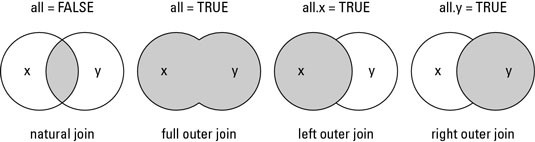
\includegraphics[width=4.16667in,height=\textheight]{figures/joins.jpg}
\caption{Join operations with \texttt{Merge()}}
\end{figure}

\end{frame}

\begin{frame}[fragile]{Joining tables}
\protect\hypertarget{joining-tables-2}{}

\begin{itemize}
\item
  If the merging key is a combination of more than one column, you can
  provide a vector to \texttt{by}.
\item
  If the columns used as key have different names in different tables,
  we need to use \texttt{by.x} and \texttt{by.y} instead of \texttt{by}.
\item
  If no \texttt{by} argument is provided, the tables are merged on the
  columns with names they both have.
\item
  \texttt{all.x}, \texttt{all.y,} and \texttt{all} are set to FALSE by
  default. This is why the default join is the natural join.
\end{itemize}

\end{frame}

\begin{frame}[fragile]{The \texttt{sqldf} package}
\protect\hypertarget{the-sqldf-package}{}

\begin{itemize}
\item
  You can run SQL queries in R using the \texttt{sqldf} package.
\item
  SQL queries must be provided to the \texttt{sqldf()} function as
  strings.
\end{itemize}

\begin{Shaded}
\begin{Highlighting}[]
\KeywordTok{library}\NormalTok{(sqldf)}
\end{Highlighting}
\end{Shaded}

\end{frame}

\begin{frame}[fragile]{Inner join with \texttt{sqldf}}
\protect\hypertarget{inner-join-with-sqldf}{}

\begin{Shaded}
\begin{Highlighting}[]
\KeywordTok{sqldf}\NormalTok{(}\StringTok{"SELECT CustomerID, Product, Price, State }
\StringTok{       FROM Sales}
\StringTok{       JOIN Clients }
\StringTok{       USING(CustomerID)}
\StringTok{       ORDER BY CustomerID"}\NormalTok{)}
\end{Highlighting}
\end{Shaded}

\begin{verbatim}
##   CustomerID Product Price State
## 1     1_2020 Toaster    38    CA
## 2     2_2019 Toaster    38    CA
## 3     2_2020      TV   407    AZ
## 4     3_2019   Radio    36    MA
\end{verbatim}

\end{frame}

\begin{frame}[fragile]{Left join with \texttt{sqldf}}
\protect\hypertarget{left-join-with-sqldf}{}

\begin{Shaded}
\begin{Highlighting}[]
\KeywordTok{sqldf}\NormalTok{(}\StringTok{"SELECT CustomerID, Product, Price, State }
\StringTok{       FROM Sales}
\StringTok{       LEFT JOIN Clients }
\StringTok{       USING(CustomerID)}
\StringTok{       ORDER BY CustomerID"}\NormalTok{)}
\end{Highlighting}
\end{Shaded}

\begin{verbatim}
##   CustomerID Product Price State
## 1     1_2019 Toaster    38  <NA>
## 2     1_2019      TV   407  <NA>
## 3     1_2020 Toaster    38    CA
## 4     2_2019 Toaster    38    CA
## 5     2_2020      TV   407    AZ
## 6     3_2019   Radio    36    MA
## 7     3_2020      TV   407  <NA>
\end{verbatim}

\end{frame}

\begin{frame}[fragile]{Cross join with \texttt{sqldf}}
\protect\hypertarget{cross-join-with-sqldf}{}

\begin{Shaded}
\begin{Highlighting}[]
\KeywordTok{sqldf}\NormalTok{(}\StringTok{"SELECT * }
\StringTok{       FROM Sales}
\StringTok{       CROSS JOIN Clients }
\StringTok{       ORDER BY CustomerID"}\NormalTok{)}
\end{Highlighting}
\end{Shaded}

\end{frame}

\begin{frame}[fragile]{Subgroup summaries with \texttt{aggregate()}}
\protect\hypertarget{subgroup-summaries-with-aggregate}{}

The \texttt{aggregate()} function can be used to compute subgroup
summary statistics.

\end{frame}

\begin{frame}[fragile]{Subgroup summaries with \texttt{aggregate()}}
\protect\hypertarget{subgroup-summaries-with-aggregate-1}{}

\begin{Shaded}
\begin{Highlighting}[]
\NormalTok{my_df <-}\StringTok{ }\KeywordTok{data.frame}\NormalTok{(}
  \DataTypeTok{age =} \KeywordTok{c}\NormalTok{(}\DecValTok{22}\NormalTok{, }\DecValTok{36}\NormalTok{, }\DecValTok{21}\NormalTok{, }\DecValTok{39}\NormalTok{, }\DecValTok{33}\NormalTok{, }\DecValTok{45}\NormalTok{, }\DecValTok{34}\NormalTok{, }\DecValTok{59}\NormalTok{),}
  \DataTypeTok{smoker =} \KeywordTok{factor}\NormalTok{(}\KeywordTok{c}\NormalTok{(}\StringTok{"no"}\NormalTok{, }\StringTok{"yes"}\NormalTok{, }\StringTok{"no"}\NormalTok{, }\StringTok{"no"}\NormalTok{, }\StringTok{"yes"}\NormalTok{,}
                    \StringTok{"no"}\NormalTok{, }\StringTok{"yes"}\NormalTok{, }\StringTok{"yes"}\NormalTok{)),}
  \DataTypeTok{child =} \KeywordTok{factor}\NormalTok{(}\KeywordTok{c}\NormalTok{(}\StringTok{"no"}\NormalTok{, }\StringTok{"yes"}\NormalTok{, }\StringTok{"no"}\NormalTok{, }\StringTok{"no"}\NormalTok{, }\StringTok{"yes"}\NormalTok{,}
                   \StringTok{"yes"}\NormalTok{, }\StringTok{"no"}\NormalTok{, }\StringTok{"yes"}\NormalTok{)),}
  \DataTypeTok{income =} \KeywordTok{c}\NormalTok{(}\FloatTok{0.8}\NormalTok{, }\FloatTok{1.8}\NormalTok{, }\FloatTok{1.6}\NormalTok{, }\FloatTok{1.5}\NormalTok{, }\FloatTok{2.3}\NormalTok{, }\FloatTok{1.4}\NormalTok{, }\FloatTok{1.8}\NormalTok{, }\FloatTok{1.5}\NormalTok{),}
  \DataTypeTok{stringsAsFactors =} \OtherTok{FALSE}\NormalTok{)}
\end{Highlighting}
\end{Shaded}

\end{frame}

\begin{frame}[fragile]{Subgroup summaries with \texttt{aggregate()}}
\protect\hypertarget{subgroup-summaries-with-aggregate-2}{}

\begin{Shaded}
\begin{Highlighting}[]
\NormalTok{my_df}
\end{Highlighting}
\end{Shaded}

\begin{verbatim}
##   age smoker child income
## 1  22     no    no    0.8
## 2  36    yes   yes    1.8
## 3  21     no    no    1.6
## 4  39     no    no    1.5
## 5  33    yes   yes    2.3
## 6  45     no   yes    1.4
## 7  34    yes    no    1.8
## 8  59    yes   yes    1.5
\end{verbatim}

\end{frame}

\begin{frame}[fragile]{Subgroup summaries with \texttt{aggregate()}}
\protect\hypertarget{subgroup-summaries-with-aggregate-3}{}

On average, do people with children earn more than people without
children?

\begin{Shaded}
\begin{Highlighting}[]
\KeywordTok{aggregate}\NormalTok{(}\DataTypeTok{formula =}\NormalTok{ income }\OperatorTok{~}\StringTok{ }\NormalTok{child,}
          \DataTypeTok{data =}\NormalTok{ my_df, }
          \DataTypeTok{FUN =}\NormalTok{ mean)}
\end{Highlighting}
\end{Shaded}

\begin{verbatim}
##   child income
## 1    no  1.425
## 2   yes  1.750
\end{verbatim}

\end{frame}

\begin{frame}[fragile]{Subgroup summaries with \texttt{aggregate()}}
\protect\hypertarget{subgroup-summaries-with-aggregate-4}{}

\begin{Shaded}
\begin{Highlighting}[]
\KeywordTok{aggregate}\NormalTok{(}
  \DataTypeTok{x =}\NormalTok{ my_df[}\StringTok{"income"}\NormalTok{],}
  \DataTypeTok{by =} \KeywordTok{list}\NormalTok{(}\DataTypeTok{child =}\NormalTok{ my_df}\OperatorTok{$}\NormalTok{child), }
  \DataTypeTok{FUN =}\NormalTok{ mean)}
\end{Highlighting}
\end{Shaded}

\begin{verbatim}
##   child income
## 1    no  1.425
## 2   yes  1.750
\end{verbatim}

\end{frame}

\begin{frame}[fragile]{Subgroup summaries with \texttt{aggregate()}}
\protect\hypertarget{subgroup-summaries-with-aggregate-5}{}

On average, do people who smoke earn more than people who don't?

\begin{Shaded}
\begin{Highlighting}[]
\KeywordTok{aggregate}\NormalTok{(income }\OperatorTok{~}\StringTok{ }\NormalTok{smoker, my_df, mean)}
\end{Highlighting}
\end{Shaded}

\begin{verbatim}
##   smoker income
## 1     no  1.325
## 2    yes  1.850
\end{verbatim}

\end{frame}

\begin{frame}[fragile]{Subgroup summaries with \texttt{aggregate()}}
\protect\hypertarget{subgroup-summaries-with-aggregate-6}{}

\begin{Shaded}
\begin{Highlighting}[]
\KeywordTok{aggregate}\NormalTok{(}
\NormalTok{  my_df[}\StringTok{"income"}\NormalTok{],}
  \KeywordTok{list}\NormalTok{(}\DataTypeTok{smoker =}\NormalTok{ my_df}\OperatorTok{$}\NormalTok{smoker), }
\NormalTok{  mean)}
\end{Highlighting}
\end{Shaded}

\begin{verbatim}
##   smoker income
## 1     no  1.325
## 2    yes  1.850
\end{verbatim}

\end{frame}

\begin{frame}[fragile]{Subgroup summaries with \texttt{aggregate()}}
\protect\hypertarget{subgroup-summaries-with-aggregate-7}{}

Is the median income higher for smokers or non-smokers?

\begin{Shaded}
\begin{Highlighting}[]
\KeywordTok{aggregate}\NormalTok{(income }\OperatorTok{~}\StringTok{ }\NormalTok{smoker, my_df, median)}
\end{Highlighting}
\end{Shaded}

\begin{verbatim}
##   smoker income
## 1     no   1.45
## 2    yes   1.80
\end{verbatim}

\end{frame}

\begin{frame}[fragile]{Subgroup summaries with \texttt{aggregate()}}
\protect\hypertarget{subgroup-summaries-with-aggregate-8}{}

\begin{Shaded}
\begin{Highlighting}[]
\KeywordTok{aggregate}\NormalTok{(}
\NormalTok{  my_df[}\StringTok{"income"}\NormalTok{],}
  \KeywordTok{list}\NormalTok{(}\DataTypeTok{smoker =}\NormalTok{ my_df}\OperatorTok{$}\NormalTok{smoker), }
\NormalTok{  median)}
\end{Highlighting}
\end{Shaded}

\begin{verbatim}
##   smoker income
## 1     no   1.45
## 2    yes   1.80
\end{verbatim}

\end{frame}

\begin{frame}[fragile]{Subgroup summaries with \texttt{aggregate()}}
\protect\hypertarget{subgroup-summaries-with-aggregate-9}{}

What is the lowest income for someone with children? And without?

\begin{Shaded}
\begin{Highlighting}[]
\KeywordTok{aggregate}\NormalTok{(income }\OperatorTok{~}\StringTok{ }\NormalTok{child, my_df, min)}
\end{Highlighting}
\end{Shaded}

\begin{verbatim}
##   child income
## 1    no    0.8
## 2   yes    1.4
\end{verbatim}

\end{frame}

\begin{frame}[fragile]{Subgroup summaries with \texttt{aggregate()}}
\protect\hypertarget{subgroup-summaries-with-aggregate-10}{}

\begin{Shaded}
\begin{Highlighting}[]
\KeywordTok{aggregate}\NormalTok{(}
\NormalTok{  my_df[}\StringTok{"income"}\NormalTok{],}
  \KeywordTok{list}\NormalTok{(}\DataTypeTok{child =}\NormalTok{ my_df}\OperatorTok{$}\NormalTok{child), }
\NormalTok{  min)}
\end{Highlighting}
\end{Shaded}

\begin{verbatim}
##   child income
## 1    no    0.8
## 2   yes    1.4
\end{verbatim}

\end{frame}

\begin{frame}[fragile]{Subgroup summaries with \texttt{aggregate()}}
\protect\hypertarget{subgroup-summaries-with-aggregate-11}{}

Is the average age of people with children higher than that of people
without children?

\begin{Shaded}
\begin{Highlighting}[]
\KeywordTok{aggregate}\NormalTok{(age }\OperatorTok{~}\StringTok{ }\NormalTok{child, my_df, mean)}
\end{Highlighting}
\end{Shaded}

\begin{verbatim}
##   child   age
## 1    no 29.00
## 2   yes 43.25
\end{verbatim}

\end{frame}

\begin{frame}[fragile]{Subgroup summaries with \texttt{aggregate()}}
\protect\hypertarget{subgroup-summaries-with-aggregate-12}{}

\begin{Shaded}
\begin{Highlighting}[]
\KeywordTok{aggregate}\NormalTok{(}
\NormalTok{  my_df[}\StringTok{"age"}\NormalTok{],}
  \KeywordTok{list}\NormalTok{(}\DataTypeTok{child =}\NormalTok{ my_df}\OperatorTok{$}\NormalTok{child), }
\NormalTok{  mean)}
\end{Highlighting}
\end{Shaded}

\begin{verbatim}
##   child   age
## 1    no 29.00
## 2   yes 43.25
\end{verbatim}

\end{frame}

\begin{frame}[fragile]{Subgroup summaries with \texttt{aggregate()}}
\protect\hypertarget{subgroup-summaries-with-aggregate-13}{}

Is the median age of smokers higher than that of non-smokers?

\begin{Shaded}
\begin{Highlighting}[]
\KeywordTok{aggregate}\NormalTok{(age }\OperatorTok{~}\StringTok{ }\NormalTok{smoker, my_df, median)}
\end{Highlighting}
\end{Shaded}

\begin{verbatim}
##   smoker  age
## 1     no 30.5
## 2    yes 35.0
\end{verbatim}

\end{frame}

\begin{frame}[fragile]{Subgroup summaries with \texttt{aggregate()}}
\protect\hypertarget{subgroup-summaries-with-aggregate-14}{}

\begin{Shaded}
\begin{Highlighting}[]
\KeywordTok{aggregate}\NormalTok{(}
\NormalTok{  my_df[}\StringTok{"age"}\NormalTok{],}
  \KeywordTok{list}\NormalTok{(}\DataTypeTok{smoker =}\NormalTok{ my_df}\OperatorTok{$}\NormalTok{smoker), }
\NormalTok{  median)}
\end{Highlighting}
\end{Shaded}

\begin{verbatim}
##   smoker  age
## 1     no 30.5
## 2    yes 35.0
\end{verbatim}

\end{frame}

\begin{frame}[fragile]{Subgroup summaries with \texttt{aggregate()}}
\protect\hypertarget{subgroup-summaries-with-aggregate-15}{}

Compare the age of the younger person with children with the age of the
younger person without chilren:

\begin{Shaded}
\begin{Highlighting}[]
\KeywordTok{aggregate}\NormalTok{(age }\OperatorTok{~}\StringTok{ }\NormalTok{child, my_df, min)}
\end{Highlighting}
\end{Shaded}

\begin{verbatim}
##   child age
## 1    no  21
## 2   yes  33
\end{verbatim}

\end{frame}

\begin{frame}[fragile]{Subgroup summaries with \texttt{aggregate()}}
\protect\hypertarget{subgroup-summaries-with-aggregate-16}{}

\begin{Shaded}
\begin{Highlighting}[]
\KeywordTok{aggregate}\NormalTok{(}
\NormalTok{  my_df[}\StringTok{"age"}\NormalTok{],}
  \KeywordTok{list}\NormalTok{(}\DataTypeTok{child =}\NormalTok{ my_df}\OperatorTok{$}\NormalTok{child), }
\NormalTok{  min)}
\end{Highlighting}
\end{Shaded}

\begin{verbatim}
##   child age
## 1    no  21
## 2   yes  33
\end{verbatim}

\end{frame}

\begin{frame}[fragile]{Subgroup summaries with \texttt{aggregate()}}
\protect\hypertarget{subgroup-summaries-with-aggregate-17}{}

What is the age of the older smoker?

\begin{Shaded}
\begin{Highlighting}[]
\KeywordTok{subset}\NormalTok{(}
  \KeywordTok{aggregate}\NormalTok{(age }\OperatorTok{~}\StringTok{ }\NormalTok{smoker, my_df, max),}
\NormalTok{  smoker }\OperatorTok{==}\StringTok{ "yes"}\NormalTok{, }
  \DataTypeTok{select =} \StringTok{"age"}
\NormalTok{  )}
\end{Highlighting}
\end{Shaded}

\begin{verbatim}
##   age
## 2  59
\end{verbatim}

\end{frame}

\begin{frame}[fragile]{Subgroup summaries with \texttt{aggregate()}}
\protect\hypertarget{subgroup-summaries-with-aggregate-18}{}

\begin{Shaded}
\begin{Highlighting}[]
\KeywordTok{subset}\NormalTok{(}
  \KeywordTok{aggregate}\NormalTok{(}
\NormalTok{    my_df[}\StringTok{"age"}\NormalTok{],}
    \KeywordTok{list}\NormalTok{(}\DataTypeTok{smoker =}\NormalTok{ my_df}\OperatorTok{$}\NormalTok{smoker), }
\NormalTok{    max),}
\NormalTok{  smoker }\OperatorTok{==}\StringTok{ "yes"}\NormalTok{,}
  \DataTypeTok{select =} \StringTok{"age"}\NormalTok{)}
\end{Highlighting}
\end{Shaded}

\begin{verbatim}
##   age
## 2  59
\end{verbatim}

\end{frame}

\begin{frame}[fragile]{Subgroup summaries with \texttt{aggregate()}}
\protect\hypertarget{subgroup-summaries-with-aggregate-19}{}

We can divide our subgroups further into more subgroups:

\begin{Shaded}
\begin{Highlighting}[]
\KeywordTok{aggregate}\NormalTok{(income }\OperatorTok{~}\StringTok{ }\NormalTok{smoker }\OperatorTok{+}\StringTok{ }\NormalTok{child, my_df, mean)}
\end{Highlighting}
\end{Shaded}

\begin{verbatim}
##   smoker child   income
## 1     no    no 1.300000
## 2    yes    no 1.800000
## 3     no   yes 1.400000
## 4    yes   yes 1.866667
\end{verbatim}

\end{frame}

\begin{frame}[fragile]{Subgroup summaries with \texttt{aggregate()}}
\protect\hypertarget{subgroup-summaries-with-aggregate-20}{}

\begin{Shaded}
\begin{Highlighting}[]
\KeywordTok{aggregate}\NormalTok{(}
\NormalTok{  my_df[}\StringTok{"income"}\NormalTok{],}
  \KeywordTok{list}\NormalTok{(}\DataTypeTok{smoker =}\NormalTok{ my_df}\OperatorTok{$}\NormalTok{smoker,}
       \DataTypeTok{child =}\NormalTok{ my_df}\OperatorTok{$}\NormalTok{child), }
\NormalTok{  mean)}
\end{Highlighting}
\end{Shaded}

\begin{verbatim}
##   smoker child   income
## 1     no    no 1.300000
## 2    yes    no 1.800000
## 3     no   yes 1.400000
## 4    yes   yes 1.866667
\end{verbatim}

\end{frame}

\begin{frame}[fragile]{Subgroup summaries with \texttt{aggregate()}}
\protect\hypertarget{subgroup-summaries-with-aggregate-21}{}

On average, do parents who smoke earn more than parents who don't smoke?

\begin{Shaded}
\begin{Highlighting}[]
\KeywordTok{subset}\NormalTok{(}
  \KeywordTok{aggregate}\NormalTok{(income }\OperatorTok{~}\StringTok{ }\NormalTok{smoker }\OperatorTok{+}\StringTok{ }\NormalTok{child, my_df, mean),}
\NormalTok{  child }\OperatorTok{==}\StringTok{ "yes"}\NormalTok{,}
  \DataTypeTok{select =} \KeywordTok{c}\NormalTok{(smoker, income)}
\NormalTok{  )}
\end{Highlighting}
\end{Shaded}

\begin{verbatim}
##   smoker   income
## 3     no 1.400000
## 4    yes 1.866667
\end{verbatim}

\end{frame}

\begin{frame}[fragile]{Subgroup summaries with \texttt{aggregate()}}
\protect\hypertarget{subgroup-summaries-with-aggregate-22}{}

\begin{Shaded}
\begin{Highlighting}[]
\KeywordTok{subset}\NormalTok{(}
  \KeywordTok{aggregate}\NormalTok{(}
\NormalTok{    my_df[}\StringTok{"income"}\NormalTok{],}
    \KeywordTok{list}\NormalTok{(}\DataTypeTok{smoker =}\NormalTok{ my_df}\OperatorTok{$}\NormalTok{smoker, }
         \DataTypeTok{child =}\NormalTok{ my_df}\OperatorTok{$}\NormalTok{child), }
\NormalTok{    mean),}
\NormalTok{  child }\OperatorTok{==}\StringTok{ "yes"}\NormalTok{,}
  \DataTypeTok{select =} \KeywordTok{c}\NormalTok{(smoker, income)}
\NormalTok{  )}
\end{Highlighting}
\end{Shaded}

\begin{verbatim}
##   smoker   income
## 3     no 1.400000
## 4    yes 1.866667
\end{verbatim}

\end{frame}

\begin{frame}[fragile]{Subgroup summaries with \texttt{aggregate()}}
\protect\hypertarget{subgroup-summaries-with-aggregate-23}{}

Is the median age of parents who smoke higher than that of parents who
don't smoke?

\begin{Shaded}
\begin{Highlighting}[]
\KeywordTok{subset}\NormalTok{(}
  \KeywordTok{aggregate}\NormalTok{(age }\OperatorTok{~}\StringTok{ }\NormalTok{smoker }\OperatorTok{+}\StringTok{ }\NormalTok{child, my_df, median),}
\NormalTok{  child }\OperatorTok{==}\StringTok{ "yes"}\NormalTok{,}
  \DataTypeTok{select =} \KeywordTok{c}\NormalTok{(smoker, age)}
\NormalTok{  )}
\end{Highlighting}
\end{Shaded}

\begin{verbatim}
##   smoker age
## 3     no  45
## 4    yes  36
\end{verbatim}

\end{frame}

\begin{frame}[fragile]{Subgroup summaries with \texttt{aggregate()}}
\protect\hypertarget{subgroup-summaries-with-aggregate-24}{}

\begin{Shaded}
\begin{Highlighting}[]
\KeywordTok{subset}\NormalTok{(}
  \KeywordTok{aggregate}\NormalTok{(}
\NormalTok{    my_df[}\StringTok{"age"}\NormalTok{],}
    \KeywordTok{list}\NormalTok{(}\DataTypeTok{smoker =}\NormalTok{ my_df}\OperatorTok{$}\NormalTok{smoker, }
         \DataTypeTok{child =}\NormalTok{ my_df}\OperatorTok{$}\NormalTok{child), }
\NormalTok{    median),}
\NormalTok{  child }\OperatorTok{==}\StringTok{ "yes"}\NormalTok{,}
  \DataTypeTok{select =} \KeywordTok{c}\NormalTok{(smoker, age)}
\NormalTok{  )}
\end{Highlighting}
\end{Shaded}

\begin{verbatim}
##   smoker age
## 3     no  45
## 4    yes  36
\end{verbatim}

\end{frame}

\begin{frame}[fragile]{Subgroup summaries with \texttt{sqldf()}}
\protect\hypertarget{subgroup-summaries-with-sqldf}{}

On average, do people with children earn more than people without
children?

\begin{Shaded}
\begin{Highlighting}[]
\KeywordTok{sqldf}\NormalTok{(}
  \StringTok{"SELECT child, AVG(income) as income }
\StringTok{  FROM my_df}
\StringTok{  GROUP BY child"}
\NormalTok{)}
\end{Highlighting}
\end{Shaded}

\begin{verbatim}
##   child income
## 1    no  1.425
## 2   yes  1.750
\end{verbatim}

\end{frame}

\begin{frame}[fragile]{Subgroup summaries with \texttt{sqldf()}}
\protect\hypertarget{subgroup-summaries-with-sqldf-1}{}

On average, do people who smoke earn more than people who don't?

\begin{Shaded}
\begin{Highlighting}[]
\KeywordTok{sqldf}\NormalTok{(}
  \StringTok{"SELECT smoker, AVG(income) as income }
\StringTok{  FROM my_df}
\StringTok{  GROUP BY smoker"}
\NormalTok{)}
\end{Highlighting}
\end{Shaded}

\begin{verbatim}
##   smoker income
## 1     no  1.325
## 2    yes  1.850
\end{verbatim}

\end{frame}

\begin{frame}[fragile]{Subgroup summaries with \texttt{sqldf()}}
\protect\hypertarget{subgroup-summaries-with-sqldf-2}{}

What is the lowest income for someone with children? And without?

\begin{Shaded}
\begin{Highlighting}[]
\KeywordTok{sqldf}\NormalTok{(}
  \StringTok{"SELECT child, min(income) as income }
\StringTok{  FROM my_df}
\StringTok{  GROUP BY child"}
\NormalTok{)}
\end{Highlighting}
\end{Shaded}

\begin{verbatim}
##   child income
## 1    no    0.8
## 2   yes    1.4
\end{verbatim}

\end{frame}

\begin{frame}[fragile]{Subgroup summaries with \texttt{sqldf()}}
\protect\hypertarget{subgroup-summaries-with-sqldf-3}{}

Is the average age of people with children higher than that of people
without children?

\begin{Shaded}
\begin{Highlighting}[]
\KeywordTok{sqldf}\NormalTok{(}
  \StringTok{"SELECT child, AVG(age) as age }
\StringTok{  FROM my_df}
\StringTok{  GROUP BY child"}
\NormalTok{)}
\end{Highlighting}
\end{Shaded}

\begin{verbatim}
##   child   age
## 1    no 29.00
## 2   yes 43.25
\end{verbatim}

\end{frame}

\begin{frame}[fragile]{Subgroup summaries with \texttt{sqldf()}}
\protect\hypertarget{subgroup-summaries-with-sqldf-4}{}

Compare the age of the younger person with children with the age of the
younger person without chilren:

\begin{Shaded}
\begin{Highlighting}[]
\KeywordTok{sqldf}\NormalTok{(}
  \StringTok{"SELECT child, min(age) as age }
\StringTok{  FROM my_df}
\StringTok{  GROUP BY child"}
\NormalTok{)}
\end{Highlighting}
\end{Shaded}

\begin{verbatim}
##   child age
## 1    no  21
## 2   yes  33
\end{verbatim}

\end{frame}

\begin{frame}[fragile]{Subgroup summaries with \texttt{sqldf()}}
\protect\hypertarget{subgroup-summaries-with-sqldf-5}{}

What is the age of the older smoker?

\begin{Shaded}
\begin{Highlighting}[]
\KeywordTok{sqldf}\NormalTok{(}
  \StringTok{"SELECT max(age) as age }
\StringTok{  FROM my_df}
\StringTok{  GROUP BY smoker}
\StringTok{  HAVING smoker = 'yes'}
\StringTok{  "}
\NormalTok{)}
\end{Highlighting}
\end{Shaded}

\begin{verbatim}
##   age
## 1  59
\end{verbatim}

\end{frame}

\begin{frame}[fragile]{Subgroup summaries with \texttt{aggregate()}}
\protect\hypertarget{subgroup-summaries-with-aggregate-25}{}

We can divide our subgroups further into more subgroups:

\begin{Shaded}
\begin{Highlighting}[]
\KeywordTok{sqldf}\NormalTok{(}
  \StringTok{"SELECT smoker, AVG(income) as income}
\StringTok{  FROM my_df}
\StringTok{  GROUP BY child, smoker}
\StringTok{  "}
\NormalTok{)}
\end{Highlighting}
\end{Shaded}

\begin{verbatim}
##   smoker   income
## 1     no 1.300000
## 2    yes 1.800000
## 3     no 1.400000
## 4    yes 1.866667
\end{verbatim}

\end{frame}

\begin{frame}[fragile]{Subgroup summaries with \texttt{sqldf()}}
\protect\hypertarget{subgroup-summaries-with-sqldf-6}{}

On average, do parents who smoke earn more than parents who don't smoke?

\begin{Shaded}
\begin{Highlighting}[]
\KeywordTok{sqldf}\NormalTok{(}
  \StringTok{"SELECT smoker, AVG(income) as income}
\StringTok{  FROM my_df}
\StringTok{  GROUP BY child, smoker}
\StringTok{  HAVING child = 'yes'}
\StringTok{  "}
\NormalTok{)}
\end{Highlighting}
\end{Shaded}

\begin{verbatim}
##   smoker   income
## 1     no 1.400000
## 2    yes 1.866667
\end{verbatim}

\end{frame}

\end{document}
